\documentclass[12pt,a4paper]{article}
\usepackage[
	left 	= 2.54cm,
	right 	= 2.54cm, 
	top 		= 2.54cm,
	bottom 	= 2.54cm,
]{geometry}
\usepackage[utf8]{inputenc}
\usepackage[english]{babel}
\usepackage[OT1]{fontenc}
\usepackage{amsmath}
\usepackage{mathtools}
\usepackage{lscape}
\usepackage{graphicx}
\usepackage{caption}
\usepackage{amssymb}
\usepackage{tikz}
\usepackage{float}


% Packages for Tables -----
\usepackage{multirow}
\usepackage{booktabs}
\usepackage[justification=centering]{caption} % Centers the caption
\usepackage{makecell}
\usepackage{lscape}
\usepackage{adjustbox}
\usepackage{longtable}

% -----

% Colorbox for Notes ------
\usepackage{tcolorbox}
\usepackage{xcolor}
\definecolor{lightblue}{RGB}{173,216,230}

\newenvironment{lightbluebox}{%
    \begin{tcolorbox}[colback=lightblue, colframe=lightblue, fontupper=\itshape]%
}{%
    \end{tcolorbox}%
}
%---------------------------

\usepackage[style=apa, backend=biber]{biblatex}
\addbibresource[]{ref.bib}
\renewcommand{\baselinestretch}{1.25} 

\usepackage[hidelinks]{hyperref}
\hypersetup{
	colorlinks = true,
	urlcolor   = blue,
	linkcolor  = black, 
	citecolor  = blue, 
}

\definecolor{green1}{HTML}{2CA02C}
\definecolor{blue1}{HTML}{1F77B4}
\definecolor{red1}{HTML}{D62728}
\definecolor{orange1}{HTML}{FF7F0E}


\usepackage{fancyhdr}
\pagestyle{fancy}
\lhead{\slshape Unterweger}
\chead{}
\rhead{\slshape \nouppercase{\leftmark}}

\usepackage{titlesec,xcolor}
\titleformat{\section}{\bfseries}{\thesection}{0.5em}{}
\titlespacing{\section}{0pt}{3ex plus 1ex minus 0.2ex}{10pt}
\setlength{\headheight}{14.49998pt}

\usepackage{titlesec,xcolor}
\titleformat{\subsection}{\bfseries}{\thesubsection}{0.5em}{}
\titlespacing{\subsection}{0pt}{3ex plus 1ex minus 0.2ex}{10pt}
\setlength{\headheight}{14.49998pt}

%% Command Overrides
\newcommand{\norm}[1]{\left\lVert#1\right\rVert}
\DeclareMathOperator*{\argmax}{arg\,max}
\DeclareMathOperator*{\argmin}{arg\,min}
\newcommand{\MC}{\textbf{(Missing Citation)}} %Command to signal missing citations



%------------------------------------------------------------------%

\author{Lucas Paul Unterweger}
\title{On the Duality of Frequentist Point Estimates and Bayesian Shrinkage Priors: An Extension based on the Triple-Gamma-Prior}


\begin{document}

\begin{titlepage}
\center
\vfill

\includegraphics[scale=0.1]{WU.png}
\vfill
\begin{tabular}[t]{lc}
Student-ID:  & 11913169 \\
Degree Program: & 
Master of Science in Economics (Science Track) \\
Examiner: & Peter Knaus, PhD \\
Submission date: & TBA \\
\end{tabular}
\vfill
{\large \textbf{Triple-Gamma-Regularization} \\
\normalsize \textit{A Flexible Non-Convex Regularization Penalty based on the Triple-Gamma-Prior}}

% Old Title
%\textit{or}\\ \textbf{On the Duality of Frequentist Point Estimates and Bayesian %Shrinkage Priors}\\
%\normalsize \textit{An Extension based on the Triple-Gamma-Prior}}

\vfill
by\\ \vspace{3mm}
{\Large Lucas Unterweger \href{https://github.com/therealLucasPaul}{
\includegraphics[scale=0.01]{GitHub.png}}}\\
(Student-ID: 11913169)\\
\vfill

\thispagestyle{empty}
\pagebreak
\end{titlepage}
\newcounter{savepage}
\pagenumbering{roman}
\thispagestyle{empty}

\begin{abstract}
\begin{lightbluebox}
Add abstract as soon as the thesis is 100\% finished.
\end{lightbluebox}
\end{abstract}

\clearpage

\section*{Acknowledgements}
\thispagestyle{empty}

This completion oft his thesis would not have been possible without so many amazing people in my life who supported me throughout the process of writing this master's thesis and the master program as a whole. I want to thank my mum, Daniela, and my dad, Werner, who always picked me up when I lost my motivation to continue and who convinced me to keep going time after time. I want to thank my brother, Tobias, who always readily listened to me complaining for hours and hours on end about things he probably barely understood and yet always agreed with me about my computational issues while doing the simulations. And most of all I want to thank my advisor, Peter, who always supported me from the day I randomly dropped an e-mail into his e-mail inbox about becoming his tutor in econometrics, although not having met once during the distance learning phase of the COVID pandemic, up until today. From working as a tutor in his team, writing a bachelor thesis, and to the support during this master thesis now. Even though sometimes living 12h time differences apart, one in Boston the other in Manila, he always answered any questions I had and supported me in whatever way he could and I want to sincerely thank him for that!  

\clearpage

\thispagestyle{plain}
\tableofcontents
\pagebreak
\setcounter{savepage}{\arabic{page}}
\pagenumbering{arabic}

\pagebreak
%----- Introduction -----
\section{Introduction}
Willam of Ockham, born in Ockham, Surrey, probably lived between 1287 and 1348 and is nowadays recognized as a pre-eminent philosopher of the middle ages. Although     his name itself is no common knowledge, a principle carrying his name is: \textit{Ockham's Razor}. Interestingly, the main formulation of the principle (\textit{Entia non sunt multiplicanda praeter necessitatem} [plurality should not be posited without necessity]) can not be traced back to Ockham directly, but variations of it can be found in Ockham's writings. Since then nonetheless, the principle has long been used by statisticians and other researchers as a a scientific credo to capture the notion that "the simpler of two explanations is to be preferred" \parencite{Lazar2010}. Recent decades and its advancements in information technology have opened the gates to seemingly unlimited amounts of data and information. Whether it is data about the carbon dioxide levels near bus stations in a city, the intraday trading volume of a specific financial asset or the rhythm of a beating heart throughout a day, new techniques and approaches in measuring digital and natural phenomena have enables researchers all around the globe to study previously unknown effects, test novel hypotheses and find relationships between real world process that would have otherwise remained hidden from the eye of human civilization.\\

Yet, these advancements come at a cost. Conventional statistical models like the \textit{ordinary least squares (OLS)} have troubles handling statistical problem in higher dimensions. When the relative number of features to the number of data points in a statistical model is very high, the estimates of these models suffer from high variance and thus generalize poorly. Frequentist statisticians have developed penalized regression approaches to battle these issues by incorporating a penalty term into the optimization problems used to estimate the coefficients of linear models. In recent decades, various penalty terms have been published with each of its own advantages and disadvantages, yet to this day no a single method has emerged to triumph above them all \parencite{WangEtAl2020}.\\

Bayesian statisticians have developed their own tools to handle high-dimensional statistical problems and commonly use specific probability distributions to battle model complexity by shrinking the estimates of less important variables towards zero (thus the name \textit{shrinkage prior}). Although these two fields of statistical thought use different approaches to tackle the same problem, a striking mathematical connection exists between those two methods. A bridge which allows mathematicians to derive a regularization penalty from specific prior distributions, which raises the question: "Does there exist a already known prior distribution in the Bayesian setting which can be used to derive a regularization penalty which might perform better than existing penalties?".\\

A prior distribution which might have these suitable properties is the unifying shrinkage prior developed by \textcite{TGP2020} called \textit{Triple-Gamma-Prior}. Its unifying properties and the fact that a closed-form solution for the marginal prior exists might lead to favourable properties in the realm of frequentist statistics, but before that it is necessary to have a closer look at what the exact problem is that Bayesian shrinkage prior and regularization approaches are trying to solve. An overview of this along with a theoretical basis of the necessary concepts will be presented in section 2.\\

The remaining thesis is structure as follows: Section 3 will provide a literature review about the history of regularization and advancements in the field along with an overview of established concepts and their respective advantages and disadvantages. Section 4 will quickly discuss the mathematical building block for this thesis by showcasing the bridge between regularization and Bayesian shrinkage prior as well as introduce the Triple-Gamma-Prior by \textcite{TGP2020} as the shrinkage prior of choice. Section 5 will then derive the proposed penalty by utilizing the bridge explained in section 4. Section 6 will then apply the newly derived regularization penalty and apply it in the context of a simulation study to see its effects and possible fields of application. The remaining sections 7 and 8 will discuss shortcomings of the method and possible extensions and end with a summarizing conclusion. 

%----- Theoretical Section
\newpage
\section{Theoretical Section}\label{sec:theorysuper}
Generally speaking, a major part of statistical learning deals with trying to describe a certain output variable $Y$ with a set of input variables $X_1, \cdots, X_p$ by trying to find a functional form $f$ which uses the given information in the inputs and - ideally - describes the hidden relationship between $Y$ and the inputs $X_i$ as accurately as possible. However, it comes as no surprise that the functional form $f$ depends on the statistical problem at hand. What type of data has been collected? Are we assuming a linear or non-linear relationship between the predictors? How much data is available and can its quality be guaranteed? But more importantly, it is necessary to ask the question whether the goal of the statistical learning method is \textit{inference} or \textit{prediction}.\\

The first of these two goals - \textit{inference} - aims at understanding the relationship that may or may not exist between the input variables $X_i$ and the output $Y$. Especially applied sciences like Economics, Psychology and Medicine often try to find a (causal) relationship within their theoretical framework to evaluate a policy, a medication or a new form of therapy. Linear models for example often provide a simple and straightforward framework which provide the scientist with interpretable effects. \textit{Prediction} on the other hand aims at forecasting the output variable $Y$ as accurately as possible and using every bit of information that is available, but disregards interpretability. \parencite[21]{ESL2009} These goals can be summarized by viewing it as a decision between \textit{prediction accuracy} and \textit{model interpretability}, which has thoroughly been explained by \textcite{ESL2009}.\\

For the purpose of this thesis, the following chapters will restrict itself to the case of linear models, hence where assume that the functional form $f$ is linear in its inputs. The commonly known \textit{least squares estimator} is one way of estimating such a functional form and due to its many desirable properties has gained popularity in various  scientific fields. 

\subsection{Model Complexity and the Problem of Under- and Overfitting}

In supervised learning, a model is fitted on an observed dataset where both inputs and outputs are given in pairs. Using this data a statistical model aims to find a functional form which maps these inputs into the output space and thus describes a relationship between those two spaces. Naturally, one would assume to find a functional form which manages to describe the relationship as closely as possible by minimizing a chosen loss function. Yet, this often ignores a problem called "overfitting" which can loosely be described as using "too much information" from the training dataset. As described by \textcite{Ying2019}, this problem arises from the fact "that over-fitted model has difficulty coping with pieces of the information in the testing set, which may be different from those in the training set". A more formal definition of overfitting has been defined by \textcite{Mitchell1997}:\\

\textbf{Definition 2:}Given a hypothesis space $\mathcal{H}$, a hypothesis $h \in \mathcal{H}$ is said to overfit the training data if there exists some alternative hypothesis $h' \in \mathcal{H}$ such that $h$ has smaller error than $h'$ over the training examples, but $h'$ has a smaller error than $h$ over the entire distribution of instances.\\

Theoretically, this problem can emerge from a multitude of reasons. One of which being that learning every piece of information in the training dataset can lead to fitting the noise rather than fitting the underlying pattern. Another reason can be ill-chosen degrees of model complexity, because "having many hypotheses intuitively increase the risk of randomly finding a solution that learn the training set “by heart”, with limited generalization ability." \parencite{ParisRobilliardFonlupt2003}.\\  

In general, a linear regression model fitted with least squares on a sufficient amount of data points ($n \gg p$) will produce estimates which both have low bias and low variance and thus tends to perform well out of sample. However, problems arise with this approach arise when the sample size decreases, because the variance in the estimates will increase. The main idea behind this can be easily be visualized by trying to fit a polynomial curve on a two dimensional space and then altering the available sample for polynomials of different order. 
\begin{figure}
\centering
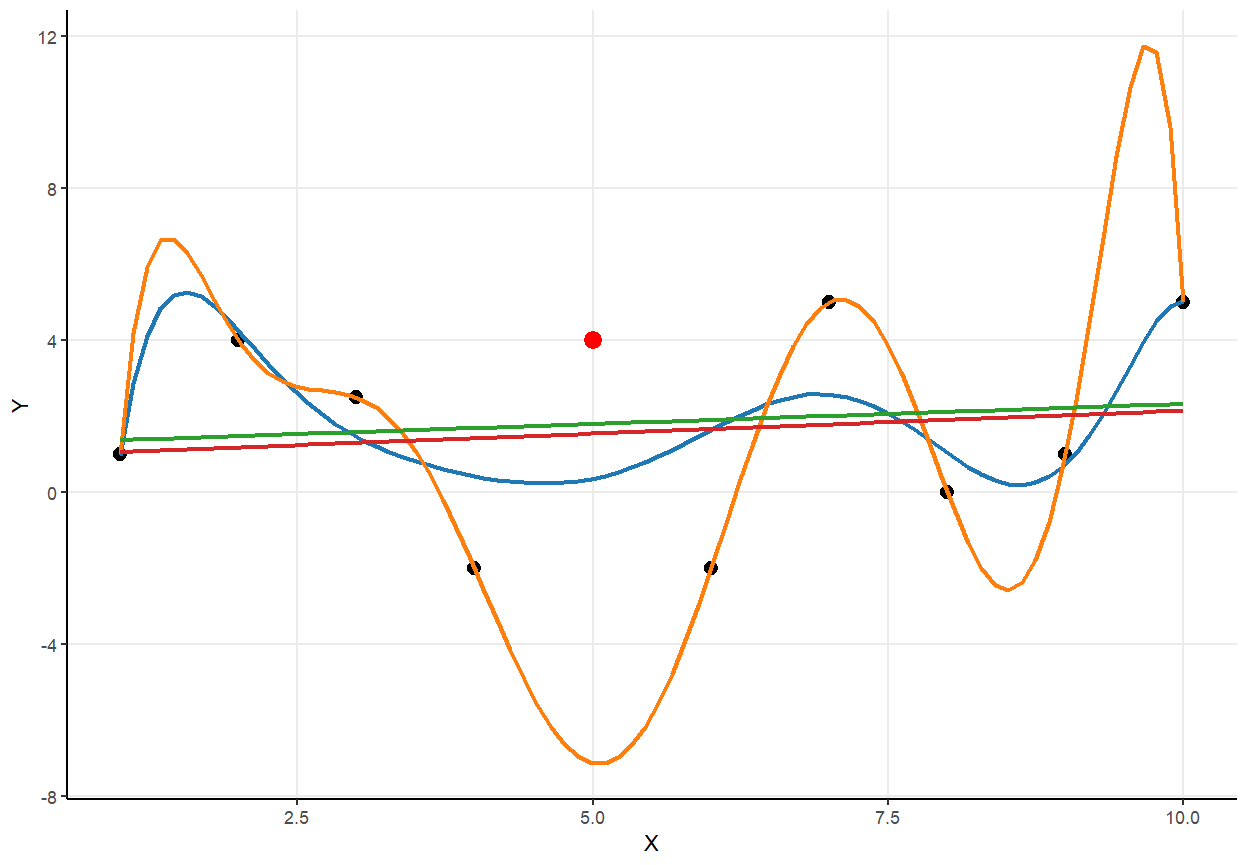
\includegraphics[scale=0.5]{PolynomialFit_Plot.png}
\caption{1st and 8th order polynomial fit to data \\ (\textcolor{green1}{Green} \& \textcolor{blue1}{Blue} Lines fitted with red data point; \textcolor{orange1}{Orange} \& \textcolor{red1}{Red} Lines fitted without).}
\label{fig:polyfit}
\end{figure}

Such a plot can be found in figure \ref{fig:polyfit}. Here, the black points represent the main data sample plotted on a two-dimensional $Y$-$X$-space. The red dot plotted at $(5,4)$ represents the additional data point which is used to alter the respective sample. Polynomials of specific orders can now be used to emulate certain levels of model complexity. For example, a first order polynomial has two coefficients to estimate: the intercept $\beta_0$ and the slope $\beta_1$. A polynomial of order of order eight has nine coefficients to estimate. What can now be seen in figure \ref{fig:polyfit} is the change in estimates if we include/exclude the additional red data point. A first-order polynomial needs at least two data points and as $n=9 > p = 2$, the overall fit of the polynomial doesn't change drastically with the additional tenth data point. In the case of the eighth-order polynomial, we need at least nine data points to create a fit as we have nine predictors (one intercept and one coefficient for each of the eight powers). In this case $n=p$ and adding another data point drastically changes the estimates coefficients, which means that the model won't perform well in out-of-sample scenarios. This emphasizes the importance a sufficient sample size when fitting linear models. And this leads us to the core field of study of this thesis: What are ways to improve the generalization of a linear model in scenarios where the sample size is not sufficiently large enough or high-dimensionality becomes a problem?\\

As already pointed out by \textcite{FanLi2006} almost 20 years ago, "high dimensional data analysis will be the most important research topic in statistics in the 21st century" and the advancements in data availability in recent decades have supported their hypothesis. The main problem to solve is how to accurately approach the problem of feature selection and make models generalize better. A first approach could be to increase the sample size to re-establish the unbiasedness of methods like OLS, however either the problem at hand involves a scenario with only few data points to begin with, or due to an extensive number of features, the collection of a sufficient amount of data points is practically not feasible. Another approach could be to use common variable selection methods like \textit{AIC} and \textit{BIC}, but as \textcite{FanLi2006} point out, "[t]raditional variable selection such as $C_p$, AIC and BIC involves a combinatorial optimization problem, which is NP-hard, with computational time increasing exponentially with the dimensionality." A third and computationally more feasible approach involves a concept called \textit{penalized regression}, more commonly known as \textit{Regularization}.

\subsubsection{Regularization}

Focusing on option three to battle model complexity, regularization methods have been studied thoroughly since the 1990s. However, the emergence of data science - and especially machine learning - as a standalone field of study has led to a broader meaning of the term \textit{regularization}. This phenomenon has been discussed by \textcite{Taxonomy2017}, where the authors establish a taxonomy to distinguish between multiple different definitions. In the traditional sense, as can be seen in \textcite[167--170]{ESL2009}, \textit{regularization} refers to a general class of problems of the form
\[
\underset{f \in \mathcal{H}}{\min}\left\{\sum_{i=1}^N L(y_i, f(x_i)) + \lambda{J}(f)\right\}
\]
where $L(.)$ refers to a loss function defined as some function of the true values and the predicted values and $J(f)$ is penalty based on the chosen functional from a space of functions $\mathcal{H}$. In the context of penalized linear regression, this is equivalent to finding the set of risk minimizing coefficients $\hat{\beta}$ from the set of all possible combinations of coefficients $\beta$. \MC Thus, resulting in the general class of regularization problems of the form:
\[
\underset{\beta \in \boldsymbol{\beta}}{\min}\left\{\sum_{i=1}^N L(y_i, f_\beta(x_i)) + \lambda{J}(\beta)\right\}
\]
where $f_\beta(x_i)$ is a linear function of the inputs $x_i$ parametrized by the coefficients $\beta$. Hence, in this setting, regularization deals with penalizing the risk function based on the value of the chosen set of coefficients. \\
However, this only describes a subset of \textit{regularization} methods as stated by \textcite{Taxonomy2017}. The authors use a more general definition of regularization:\\

\textbf{Defintion 2: Regularization} is any supplementary technique that aims at making the model generalize better, i.e. produce better results on the test set.\\

Building on that, they split up the majority of \textit{regularization} methods into  (1) methods applied to the data set like transformations or modifications of the inputs, (2) methods altering the selected model family , (3) methods applied to the error/loss function $L(y_i, f_\beta(x_i))$ , (4) methods applied to regularization/penalty term as described above and (5) alterations of the optimization procedure itself. 

Unsurprisingly, this thesis is concerned with the fourth group of regularization methods, which add a penalty/regularization term $J(\beta)$ into the risk function, but before advancing to literature that deals with this kind of problem, it is necessary to establish a terminology which will be used throughout this thesis. This terminology will be the following:

Let $\mathcal{D}$ be a training data set with $n \in \mathbb{N}$ observations, where every  consists of a target variable $y_i \in \mathbb{R}$ along with a number of corresponding inputs $x_i \in \mathbb{R}$. Given a linear function $f_\beta(x_i)$ of the inputs parametrized by coefficients $\beta \in \boldsymbol{\beta}$, $L(y_i f_\beta(x_i))$ is the \textbf{Loss} function measuring the discrepancy between the actual target $y_i$ and the output of the linear function $f_\beta(x_i)$. According to \textcite{Vapnik1991}, the \textbf{Empirical Risk Functional} is then 
\[
R_{emp}(\beta) = \frac{1}{n} \sum_{i=1}^n L(y_i, f_\beta(x_i)).
\]
\textbf{Regularization} in this thesis' context refers then to adding some penalty function $J(\beta)$ dependent on the set of parameters $\beta$, multiplied by some weighting parameter $\lambda$, to the empirical risk functional $R_{emp}(\beta)$. Thus, $R_{reg} = R_{emp}(\beta) + \lambda\cdot J(\beta)$. This results in the overall optimization problem
\begin{align}
&\underset{\beta \in \boldsymbol{\beta}}{\argmin}\left\{R_{reg}(\beta)\right\}\nonumber\\
&=\underset{\beta \in \boldsymbol{\beta}}{\argmin}\left\{R_{emp}(\beta) + \lambda\cdot J(\beta)\right\}\nonumber\\
&=\underset{\beta \in \boldsymbol{\beta}}{\argmin}\left\{\sum_{i=1}^n L(y_i, f_\beta(x_i)) + \lambda\cdot J(\beta)\right\}\label{eq:genreg}
\end{align}

It is important to note here that as $J(\beta)$ is only a function of the coefficients $\beta$ and neither the targets $y_i$ nor the inputs $x_i$. It only affects the generalization error of the model, not the training error given by the empirical risk functional $R_{emp}(\beta)$.


\subsection{Bayesian View on Battling Model Complexity using Shrinkage Priors}\label{sec:BayesianShrinkagePriors}
To build on the mathematical connection between the Bayesian and Frequentist approach to battle model complexity, which will be used as the building block of this thesis later on, it is necessary to make a quick detour and quickly recap on how Bayesian statisticians tackle model complexity. 

\begin{lightbluebox}
Explain Shrinkage Prior
\end{lightbluebox}


\newpage

%----- Literature Review -----
\section{Literature Review}\label{sec:litreview}

The concept of a penalized regression has been around for quite some time and been studied widely in various fields of scientific research. Arguably, this methodological approach to penalized regression started with the publication of two pieces of literature published by Arthur Hoerl and Robert Kennard in 1970 \parencite{HoerlKennard1970a, HoerlKennard1970b}. With these two papers the authors introduced the widely known \textit{Ridge Regression}, which has been developed from the previously known concept of Ridge analysis. In its core, the authors were trying to tackle the problem of high variances of the regression coefficients in high-dimensional problem settings. This shrinkage estimator, which uses the squared coefficient as a penalty term, "attempt[s] to shrink the coefficients to
reduce these variances, while adding some bias." \parencite{Hoerl2020} This closely resembles the previously discussed issue of the \textit{Bias-Variance-Tradeoff}, which has been discussed in the \textit{Under- and Overfitting} chapter in section \ref{sec:theorysuper} (Roger W. Hoerl, Arthur Hoerl's son, published a historical overview of the development of the concept of \textit{Ridge Regression} in 2020 \parencite{Hoerl2020}). The closed from solution of the Ridge estimator is given by
$$\hat{\beta}_{Ridge} = \left(X^TX+\lambda I\right)^{-1}X^Ty$$,
which adjusts the OLS estimator by shifting the main diagonal entries of the design matrix by $\lambda$ ($\lambda \geq 0$). It can be shown that this closed form estimator is equivalent to a Lagrangian problem of the following form \parencite{VanWieringen2015}:
$$\hat{\beta}_{Ridge}(\lambda) = \underset{\beta}{\argmin}\left\{\norm{y-X\beta}_2^2 + \lambda\norm{\beta}_2^2\right\}$$
This resembles an example of the above defined regularization framework with squared residual loss and a penalty term of the form $\norm{\beta}_2^2$, which only depends on the parameter $\beta$. In case of $\lambda$ being equal to zero, this reduces to the \textit{maximum likelihood (ML) estimator}. 

The publications of Arthur Hoerl and Robert Kennard have led to further advancements, although it took more than 25 years, in shrinkage estimation or related concepts. One concept which is almost as famous \textit{Ridge Regression} is the \textit{Least Absolute Shrinkage and Selection Operator}, more commonly know as \textit{LASSO}, developed by \textcite{Tibishirani1996}. He argues that the two at the time most prominent shrinkage methods - Ridge and Subset Selection - both have their drawbacks. Ridge regression on the one hand is an optimization problem which continuously shrinks coefficients towards zero, but doesn't select them in a discrete sense, which makes it hard to interpret these models. Subset Selection on the other hand chooses variables in a discrete sense - a variables either stays within the model or it doesn't - and thus creates easily interpretable models, but "[s]mall changes in the data can result in very different models being selected and this can reduce its prediction accuracy." \parencite{Tibishirani1996} \textit{LASSO} is trying to combine both methods' advantages by using $\norm{\beta}_1$ as a penalty term.\\

\textit{LASSO} and to some extend \textit{Ridge} can be viewed as a special case of a $l_p$-norm regularization with corresponding values for $p$ ($p = 1$ for LASSO and $p=2$ for Ridge) \parencite{FrankFriedman1993}. 

$$\norm{\beta}_p =  \left(\sum_{i=1}^p|\beta_i|^p\right)^{1/p}$$

Work published by researchers in the nineties, like the previously mentioned \textcite{FrankFriedman1993} or \textcite{Fu1998}, as well as more recent literature like \textcite{WangEtAl2020} have repeatedly shown there is no go-to-method to tackle regularization problems, as the effectiveness of a specific approach highly depends on the data siuation at hand. Due to this particular situation in the literature, several other methods have been proposed in the recent years and decades. An approach combining \textit{Ridge} and \textit{LASSO} two methods is called \textit{Elastic Net} regularization and has been developed by \textcite{ZouHastie2005}. The authors there elaborate on some of the shortcomings of the LASSO method. For example, in a special case where there are more predictors $p$ than data points $n$ ($p > n$), LASSO only selects up to $n$ variables due to the nature of the convex optimization problem. Should several of the included variables be highly \textit{pairwise} correlated with each other, \textit{LASSO} tends to only select on of these variables. In its core, \textit{Elastic Net Regularization} linearly combines the penalty terms of \textit{Ridge} and \textit{LASSO} regularization, yielding a loss function of the form:\\
$$J(\beta) = \lambda_1 \norm{\beta}_2^2 + \lambda_2 \norm{\beta}_1$$
The authors have	 shown that, especially when it comes to encouraging the aforementioned grouping effects, \textit{Elastic Net} tends to perform better than the \textit{LASSO}.\\

Recent years however have opened up a new subfield of approaches to regularization. Methods like \textit{LASSO, Bridge} \parencite{FrankFriedman1993}, \textit{Ridge} and \textit{Elastic Net}\footnote{Elastic Net, due to its mathematical definition, can be view as a generalization of \textit{Ridge} and \textit{LASSO}.} are convex functions in its parameters and are thus usually classified as \textit{Convex Regularization Penalties}. Recently, the literature has shifted towards penalties which are non-convex functions in its parameters, usually called \textit{Non-Convex Regularization Penalties}\footnote{Note: They are called \textit{non-convex} penalties and not \textit{concave} penalties, because non-convexity does not necessarily imply concavity.}. One recent example of such a penalty includes \textcite{JohnVettamWu2022}, who proposed a penalty structure called \textit{Gaussian penalty} and which is based on a Gaussian-like function by using $J(\beta) = 1 - e^{-\kappa\beta^2}$. Another method proposed by \textcite{WangZhu2016} is called the \textit{Atan penalty} - or \textit{Arctan} penalty - and makes use of the favourable properties of the \textit{Arctan} function by using the penalty $J(\beta, \gamma) = (\gamma + \frac{2}{\pi})\arctan(\frac{|\beta|}{\gamma})$. Several others include \textit{SCAD} \parencite{FanLi2001}, \textit{MCP} \parencite{Zhang2010} or \textit{Laplace} \parencite{TrzaskoManduca2009} penalties.\\

Seeing this vast array of different pieces of literature immediately raises the question on advantages and disadvantages of specific methods and why so many have established itself in this particular field of study. Keeping in mind that the effectiveness of a method still highly depends on the data situation at hand, it is still important to distinguish methods based on its mathematical properties. \textcite{JohnVettamWu2022} have distinguished methods based on two broad criteria: (1) How does a penalty behave in small neighbourhoods around zero? (Is it smooth or singular at origin?) and (2) Is the underlying function convex or non-convex? To better incorporate the proposed concept of this thesis into this body of literature, I am proposing a third property to distinguish penalty terms: (3) How does the function behave in the limits? (Does it converge or diverge?) \\

\begin{center}
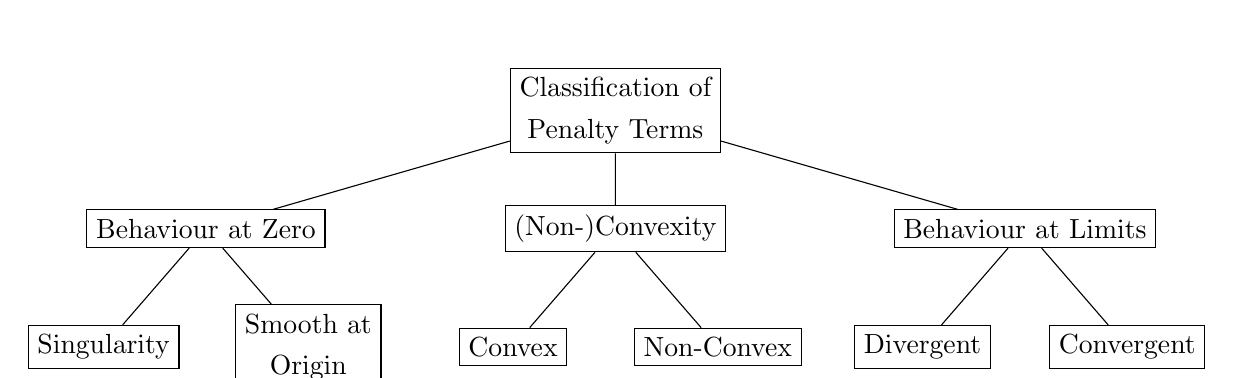
\begin{tikzpicture}[
    level 1/.style={sibling distance=5.2cm},
    level 2/.style={sibling distance=2.6cm},
    level 3/.style={sibling distance=2.6cm, level distance=2.5cm},
    every node/.style={draw, rectangle, align=center}
]
\node {Classification of \\ Penalty Terms}
    child { node {Behaviour at Zero}
        child { node {Singularity} }
        child { node {Smooth at \\ Origin}}
    }
    child { node {(Non-)Convexity}
        child { node {Convex}}
        child { node {Non-Convex}}
    }
    child { node {Behaviour at Limits}
        child { node {Divergent}}
        child { node {Convergent}}
    };
\end{tikzpicture}  
\end{center}

As already mentioned earlier in section \ref{sec:theorysuper}, a penalty function is a function dependent on the parameter of the model and it does not depend on the data at hand. Thus, changes in your data set does not effect the penalty directly, but only the overall optimization problem through the empirical risk functional $R_{emp}$. The following table classifies some of the existing concepts based on the three criteria mentioned earlier. A visualisation of them can be found in figure \ref{fig:DifferentPenalties} in chapter \ref{subsec:comparepenalties}.\\

Depending on what property a penalty has, it can perform specific tasks or provide challenges in application. As thoroughly described by \parencite{JohnVettamWu2022}, penalties with a singularity at origin tend to be suitable when the goal of the statistical analysis is variable selection but "could pose theoretical and computational challenges when the focus is on regularization alone without variable selection." In addition, it has been shown in the literature that "objective functions which are a sum of a nonconvex, singular-at-origin penalty function coupled with either a smooth nonconvex loss function or a nonsmooth convex loss function, often fails to satisfy a theoretical condition known as ‘Clarke regularity’." (A result presented in \textcite{QiCuiLiuPang2021}) 
Convex penalties are generally easier to implement using common optimization algorithms than non-convex penalties and, more importantly, penalties which are divergent and its limits, which most convex penalties are, yield biased results. Due to the fact that, when using divergent and convex penalties like LASSO and Ridge, the additional penalty for larger estimates keeps rising with estimates which deviate from zero, estimates are getting artificially pulled towards zero and are thus biased. Non-Convex penalties, which are usually convergent in its limits towards $-\infty$ and $+\infty$, tend to yield unbiased results as the additional penalty becomes zero as soon as a certain threshold is crossed (Again, referring to the visualisation in figure \ref{fig:DifferentPenalties}).

\begin{lightbluebox}
Still have to figure out how to fit this table.
\end{lightbluebox}    

\begin{table}[!h]
\begin{center}
\begin{tabular}{llccc}\toprule
 \multicolumn{2}{c}{Penalty} & \multicolumn{3}{c}{Classification}\\
		\cmidrule(r{4pt}){1-2} \cmidrule(l){3-5}
Penalty     	& Reference  & \makecell{Behaviour\\ at Origin} & (Non-)Convexity & Limits\\\midrule

LASSO 	& \textcite{Tibishirani1996}	& Singular	&	Convex 	& Divergent\\
Ridge 	& \textcite{HoerlKennard1970a}	& Smooth		& Convex			& Divergent\\
Gaussian & \textcite{JohnVettamWu2022}	& Smooth		& Non-Convex 	& Convergent\\
Ar(c)tan 	& \textcite{WangZhu2016}	& Singular 	& Non-Convex 	& Convergent\\
Elastic-Net & \textcite{ZouHastie2005} & Singular & Convex &\\
Bridge & \textcite{FrankFriedman1993}& Both &&\\
MCAP & \textcite{Zhang2010}& Singular & Non-Convex &\\
SCAD & \textcite{FanLi2001} & Singular & Non-Convex &\\
Laplace & \textcite{TrzaskoManduca2009} & Non-Convex &&\\
Triple-Gamma & - & \makecell{Depending\\ on parameters} & Non-Convex & Divergent \\

\end{tabular}
\caption{Classification of several Penalties}
\label{tab:ClassificationOfPenalties}
\end{center}
\end{table}
 
\section{Bayesian-Frequentist Duality of Ridge and LASSO Regression}

The main motivation for this thesis stems from a striking duality that exists between Bayesian shrinkage priors (discussed in chapter \ref{sec:BayesianShrinkagePriors}) and the frequentist approach using regularization. Both approaches aim at tackling the issue of model complexity and overfitting by making it necessary for the data to be more convincing that the value of an estimate is statistically significant different from zero. As mentioned, Bayesian statistics use specific prior distributions with a usually a lot of mass around zero and heavy tails, whereas frequentist statisticians usually alter their optimization problems incorporating penalty terms into into their loss functions. On a first glance, these two approaches have no immediate mathematical connection, however this turns out to be wrong.\\

In a Bayesian setting, one usually assumes that the parameter vector $\mathbb{\beta}$ has a prior distribution $p(\mathbb{\beta}$. By multiplying it with the likelihood of the data $f(y|X,\beta)$ and by utilizing Bayes' rule, one retrieves the posterior distribution of the parameter distribution, up to a proportionality constant:

$$p(\beta|y,X) \propto f(y|X, \beta) \times p(\beta)$$  

It turns out, as can be seen in \textcite[248--250]{ESL2009} and \textcite{VanWieringen2015} among others, that when choosing certain prior distributions and using standard assumptions in Bayesian modelling (ie the individual parameters of the parameter vector are independent a prior and the errors of the standard linear model are drawn from a normal distribution), that the moments of the posterior distributions correspond to the point estimates of a regularization approach in a frequentist setting. As this idea is essential to the entire thesis, a shortened derivation of this duality for the case of \textit{Ridge} regression will now be shown.\\

Assuming that a response variable $y_i$ follows a linear model with $k$ variables and errors $\epsilon_i \sim \mathcal{N}(0, \sigma^2)$, then the likelihood of the data is given by
$$\mathcal{L}(y|X,\beta)=\frac{1}{(2\pi\sigma^2)^{n/2}}\exp\left(-\frac{1}{2\sigma^2}\sum_{i=1}^n\epsilon_i^2\right).$$

Under the previously mentioned assumption that $p(\beta) = \prod_{i=1}^k$ and by choosing a Gaussian distribution with mean zero and variance $\tau^2$, we gain the prior distribution
$$p(\beta) = \frac{1}{(2\pi\tau^2)^{p/2}}\exp\left(-\frac{1}{2\tau^2}\norm{\beta}_2^2\right).$$

Putting both together using Bayes' theorem yields and taking the $\log$ of the distribution yields
$$\log(p(\beta|y,X)) \propto -\frac{1}{2\sigma^2}\sum_{i=1}^n \epsilon_i^2  - \frac{1}{2\tau^2}\norm{\beta}_2^2.$$

By viewing $\frac{1}{2\tau^2}$ as the weighting parameter $\lambda$, which controls the strength of the regularization. The \textit{maximum-a-priori} estimate $\hat{\beta}_{MAP}$, which can be viewed as trying to find the $\underset{\beta}{\argmax}$ of the $\log$-posterior, can be used to construct the following optimization problem:

$$\hat{\beta}_{MAP} = \underset{\beta}{\argmin}\left\{\frac{1}{2\sigma^2}\sum_{i=1}^n \epsilon_i^2  + \frac{1}{2\tau^2}\norm{\beta}_2^2\right\}$$

This optimization problem constitutes the connection between the Bayesian and the frequentist approach as it can be interpreted as (1) finding the mode of the posterior distribution when using a Gaussian prior distribution and (2) finding the parameters which minimize the loss when using a Ridge regression with $\lambda = 1/(2\tau^2)$. The same connection exists for the case of \textit{LASSO} regression which can be derived using the same procedure and a double-exponential - also called \textit{Laplace} - distribution with mean zero and some scale parameter $\tau$ as the prior for the parameter vector $\beta$. 

\subsection{Triple-Gamma-Prior by \textcite{TGP2020}}
This opens up a path of possibility to utilize this connection and derive a new regularization penalty by using a different shrinkage prior. Recently, a new development in the are of shrinkage priors has been made by \textcite{TGP2020}, who proposed a new shrinkage prior called the \textit{Triple-Gamma-Prior} which has several advantageous properties and also comes with a closed-form solution of the marginal prior distribution for $\beta$, which sets the building block for this thesis' research question:

\begin{quote}
Can the closed-form marginal distribution of the Triple-Gamma-Prior
be used to derive a new regularization penalty and do its advantages
carry over into the frequentist framework?
\end{quote}

Yet, before diving into the mathematical core of this thesis which derives said concept, it is necessary to have a look at the Triple-Gamma-Prior in depth to explain why this particular prior might prove itself to provide a useful building block for a novel regularization penalty.\\

As already mentioned above, BMA and shrinkage priors are two Bayesian approaches to deal with statistical problems in high-dimensional settings. The prior is generally constructed for variance selection in sparse state space and TVP models and is named the Triple-Gamma-Prior as it's representation is given by three Gamma distributions. A key advantage of this prior is its unifying property. As cam be seen in table 1 in \textcite{TGP2020}, special cases of the prior, depending on certain values in its hyperparameters, are the Normal-Exponential-Gamma, the Horseshoe and the double Gamma prior. In addition, it can also be seen as a special case of the LASSO prior. Another advantage is its function as a bridge between spike-and-slap and continuous shrinkage prior as the hyperparameters can be used both for steering the shrinkage effect on noise while also preventing overshrinking the signal. Computationally the shrinkage prior performs better than commonly used spike-and-slab priors as it is a continuous shrinkage prior which can more easily implemented using Markov-Chain-Monte-Carlo (MCMC) methods.\\ 

Mathematically, the prior builds on the work by \textcite{BittoFS2019} in which the authors introduced the \textit{double gamma prior} with the following hierarchical representation:

$$\theta_j|\xi^2_j \sim \mathcal{G}\left(\frac{1}{2}, \frac{1}{2\xi^2_j} \right), \quad \xi^2_j | a^\xi, \kappa^2_B \sim \mathcal{G}\left(a^\xi, \frac{a^\xi\kappa_B^2}{2}\right)$$

It is important to note here, that the \textit{double gamma prior} is a global-local shrinkage prior, where the global hyperparameter $\kappa^2_B$ is the same for all parameters $\theta_j$ and the local hyperparameter $\xi^2_j$ is the local component. The \textit{Triple-Gamma-Prior} now adds a third Gamma prior into this framework by replacing $\kappa_B^2$ in the second-level prior with $\kappa_j^2$, which follows
$$\kappa_j^2 | c^\xi, \kappa_B^2 \sim \mathcal{G}\left(c^\xi, \frac{c^\xi}{\kappa_B^2}\right)$$ 

The core property which is relevant to this thesis can be found in \textit{Theorem 1 (b)} in \textcite{TGP2020} which shows that the \textit{Triple-Gamma-Prior} has a closed-form marginal prior distribution for the parameter $\theta_j$, or to stick with the terminology of this thesis $\beta_j$. The prior is given by
$$p(\sqrt{\beta_j}|\phi^\xi, a^\xi, c^\xi) = \frac{\Gamma(c^\xi + \frac{1}{2})}{\sqrt{2\pi \phi^\xi}\cdot B(a^\xi, c^\xi)}\cdot U\left(c^\xi + \frac{1}{2}, \frac{3}{2}-a^\xi, \frac{\beta_j}{2\phi^\xi}\right),$$
where $\phi^\xi = \frac{2c^\xi}{\kappa^2_Ba^\xi}$ and $U(a,b,z)$ is the confluent hyper-geometric function of the second kind of \textcite{Tricomi1947} given by
$$U(a,b,z) = \frac{1}{\Gamma(a)}\int_0^\infty e^{-zt}t^{a-1}(1+t)^{b-a-1}dt$$

According to the mathematical connection described above, this prior can now be used to derive a novel regularization penalty.

\begin{lightbluebox}
Should I talk more extensively about the TGP? Is there something important I forgot to mention?
\end{lightbluebox}

%----- Model Setup and Derivation
\newpage
\section{Model Setup and Derivation}\label{sec:modelderivation}
Coming to the theoretical framework of the \textit{triple-gamma-regularization}, let's assume we have a response variable $y$ and $p$ predictors along with $n$ data points. More formally, let $y=[y_1  \quad y_2 \cdots y_n]^T$ and $x_i = [x_{i1} \quad x_{i2} \cdots x_{in}]^T$ with $\forall i\in \{1,...,n\}: y_i, x_i \in \mathbb{R}$. Here, $x_i$ is the $i$-th predictor, thus resulting in the design matrix $X = [x_1 \quad x_2 \cdots x_p]$.\\

Starting from the Bayesian framework, the standard linear regression model is given by
\[
y_i = x_i^T\cdot \beta + \varepsilon_i \quad i\in \{1,...,n\}. 
\]
with the assumed distribution of $\varepsilon_i \sim N(0,\sigma^2)$. Thus it follows that $y\sim N_n(X\beta,\sigma^2I)$. The posterior distribution of the parameter vector $\beta$, according to Bayes' Rule, is then proportional to the product of the likelihood of the data and the prior distribution, which can be seen in equation \ref{eq:bayes}.
\begin{equation}\label{eq:bayes}
p(\beta|y, X, \sigma^2) \propto \mathcal{L}(y|\beta, \sigma^2, X)\times p(\beta)
\end{equation}	

As stated above, each data point $y_i$ is assumed to be identically and independently drawn from a normal distribution with mean $X\beta$ and variance $\sigma_i^2$, thus:
\begin{align}
\mathcal{L}(\mathbf{y}|\beta, \sigma^2, X) 	&= \prod_i^n p(y_i|\beta, \sigma^2, X_i) \nonumber\\
						&= \prod_i^n \frac{1}{\sqrt{2\pi\sigma^2}} \exp\left(-\frac{1}{2}\left(\frac{x_i-\mu}{\sigma}\right)^2\right) \nonumber\\
						&= \frac{1}{(2\pi\sigma^2)^{n/2}}\exp\left(-\frac{1}{2\sigma^2}(\mathbf{y}-\mathbf{X}\beta)^\top(\mathbf{y}-\mathbf{X}\beta)\right) \label{eq:likelihood}
\end{align}

The log of the likelihood function is then given by 
\begin{align*}
\log \mathcal{L}( \mathbf{y} |\beta, \sigma^2 , \mathbf{X}) &= \log \left( \frac{1}{(2\pi\sigma^2)^{n/2}} \exp\left(-\frac{1}{2\sigma^2} (\mathbf{y} - \mathbf{X}\beta)^\top (\mathbf{y} - \mathbf{X}\beta)\right) \right) \\
&= \log \left( \frac{1}{(2\pi\sigma^2)^{n/2}} \right) + \log \exp\left(-\frac{1}{2\sigma^2} (\mathbf{y} - \mathbf{X}\beta)^\top (\mathbf{y} - \mathbf{X}\beta)\right) \\
&= -\frac{n}{2} \log(2\pi\sigma^2) - \frac{1}{2\sigma^2} (\mathbf{y} - \mathbf{X}\beta)^\top (\mathbf{y} - \mathbf{X}\beta)\\
&\propto - \frac{1}{2\sigma^2} (\mathbf{y} - \mathbf{X}\beta)^\top (\mathbf{y} - \mathbf{X}\beta) = - \frac{1}{2\sigma^2}\norm{\mathbf{y} - \mathbf{X}\beta}_2^2.\\
\end{align*}

The marginal prior distribution for the parameter vector $\beta$ stems from the Triple-Gamma-Prior constructed in \textcite{TGP2020} given in Theorem 1 (a) and is given by
\begin{align*}
p(\sqrt{\beta_j}|\phi^\xi, a^\xi, c^\xi) &= \frac{\Gamma(c^\xi + \frac{1}{2})}{\sqrt{2\pi \phi^\xi}\cdot B(a^\xi, c^\xi)}\cdot U\left(c^\xi + \frac{1}{2}, \frac{3}{2}-a^\xi, \frac{\beta_j}{2\phi^\xi}\right)\\
&\propto U\left(c^\xi + \frac{1}{2}, \frac{3}{2}-a^\xi, \frac{\beta_j}{2\phi^\xi}\right).
\end{align*}
Here, $U(a,b,z)$ refers the confluent hyper-geometric function of the second kind which was introduced by \textcite{Tricomi1947}. As this prior is specified for the parameter $\sqrt{\beta_j}$, we transform the prior by squaring the parameter to gain
\begin{align*}
p(\beta_j|\phi^\xi, a^\xi, c^\xi) &\propto U\left(c^\xi + \frac{1}{2}, \frac{3}{2}-a^\xi, \frac{\beta_j^2}{2\phi^\xi}\right).
\end{align*}
Now, assuming that the parameters are independent a priori, the prior distribution is given by
\begin{align}
p(\beta) 	&= \prod_j^p p(\beta_j) \nonumber\\
			&= \prod_j^p p(\beta_j|\phi^\xi, a^\xi, c^\xi) \nonumber\\
			&\propto \prod_j^p U\left(c^\xi + \frac{1}{2}, \frac{3}{2}-a^\xi, \frac{\beta_j^2}{2\phi^\xi}\right) \nonumber\\
			&= \prod_j^p \frac{1}{\Gamma(c^\xi + \frac{1}{2})}\int_0^\infty e^{-(\frac{\beta_j^2}{2\phi^\xi})t}t^{c^\xi + \frac{1}{2}-1}(1+t)^{\frac{3}{2}-a^\xi-c^\xi + \frac{1}{2}-1}dt \nonumber\\
			&\propto \prod_j^p \int_0^\infty \exp\left(-\frac{\beta_j^2}{2\phi^\xi}t\right)t^{c^\xi - \frac{1}{2}}(1+t)^{1-a^\xi-c^\xi} dt. \label{eq:prior}
\end{align}

Here, in line 1 the assumption of independence between the parameters has been used to describe the distribution of the parameter vector as the product of its individual parameter distributions. In line 2, the marginal prior from \textcite{TGP2020} has been used as the prior distribution for each individual parameter $\beta_j$. In line 3, scaling parameters have been removed by using the proportionality assumption. The last two lines of the derivation insert the integral representation of the confluent hyper-geometric function of the second kind, $U(a,b,z)$, which is valid in the case of a positive real part for the first parameter ($\mathfrak{Re}(a) > 0$) and again apply proportionality.\\

Taking the $\log$ of the prior distribution and using the properties of the logarithmic function yields the general result
\[
\log(p(\beta))=\log(\prod_j^p p(\beta_j|\phi^\xi, a^\xi, c^\xi))=\sum_j^p \log(p(\beta_j|\phi^\xi, a^\xi, c^\xi)).
\]

A common approach to estimation in regularization settings is the \textit{maximum a posteriori probability (MAP)} estimator, which is defined as
\[
\hat{\beta}_{MAP}(x) = \underset{\beta \in \mathbb{R}^p}{\argmax}\left\{f(x|\beta)g(\beta)\right\}.
\]
where $f(x|\beta)$ describes the the probability density function of a variable $x$, which is parametrized by the parameter vector $\beta$. The second function $g(\beta)$ incorporates our prior information about the parameter vector $\beta$ into the optimization problem.\\  

Returning to our specific problem at hand, the posterior distribution of our parameter vector $\mathbf{\beta}$ can be retrieved by applying Bayes' theorem and the previously gained results in equations \ref{eq:prior} and \ref{eq:likelihood}. Thus, the posterior distribution of the parameter vector $\beta$ is proportional to
\begin{align}
p(\beta|y, X, \sigma^2) 	&\propto p(y|X,\beta,\sigma)\times p(\beta) \nonumber\\
						&\propto \frac{1}{(2\pi\sigma^2)^{n/2}}e^{-\frac{1}{2\sigma^2}(y-X\beta)^T(y-X\beta)} \times \prod_j^p U\left(c^\xi + \frac{1}{2}, \frac{3}{2}-a^\xi, \frac{\beta_j^2}{2\phi^\xi}\right).\label{eq:posterior}
\end{align} 

Making use of the monotonicity of the logarithmic function and seeing that it is easier to optimize the log-posterior, Taking the log of the posterior probability distribution, we take the log of result \ref{eq:posterior}. 
\begin{align}
\log(\beta| X, y, \sigma^2) 	&= \log\left(\frac{1}{(2\pi\sigma^2)^{n/2}}\right) - \frac{1}{2\sigma^2}\norm{\mathbf{y} - \mathbf{X}\beta}_2^2 + \log\left(\prod_j^p U\left(c^\xi + \frac{1}{2}, \frac{3}{2}-a^\xi, \frac{\beta_j^2}{2\phi^\xi}\right)\right)\nonumber\\
							&= \log\left(\frac{1}{(2\pi\sigma^2)^{n/2}}\right) - \frac{1}{2\sigma^2}\norm{\mathbf{y} - \mathbf{X}\beta^2}_2^2 + \sum_j^p \log\left(U\left(c^\xi + \frac{1}{2}, \frac{3}{2}-a^\xi, \frac{\beta_j}{2\phi^\xi}\right)\right)\nonumber\\
							&\propto -\frac{1}{2\sigma^2}\norm{\mathbf{y} - \mathbf{X}\beta}_2^2 + \sum_j^p \log\left(U\left(c^\xi + \frac{1}{2}, \frac{3}{2}-a^\xi, \frac{\beta_j^2}{2\phi^\xi}\right)\right)\nonumber
\end{align}

To align with the general specification structure of regularization problems, which can be seen from equation \ref{eq:genreg}, a parameter $\lambda$ will be multiplicatively added in front of the penalty term, which makes it possible to adjust the strength of the influence that the penalty has on the chosen parameters. By minimizing the negative log-posterior adjusted with $\lambda$, we can retrieve the \textit{maximum a posteriori probability (MAP)} estimator using \textbf{Triple-Gamma-Regularization}:
\begin{equation}\label{eq:tgr}
\hat{\beta}_{MAP} = \underset{\beta \in \mathbb{R}^p}{\argmin} \left(\frac{1}{2\sigma^2}\norm{\mathbf{y} - \mathbf{X}\beta}_2^2 + \lambda \sum_j^p -\log\left(U\left(c^\xi + \frac{1}{2}, \frac{3}{2}-a^\xi, \frac{\beta_j^2}{2\phi^\xi}\right)\right)\right) 
\end{equation}

\newpage
\subsection{Varying the Hyperparameters}
After closer inspection of equation \ref{eq:tgr}, it can easily be seen that this resembles the general penalized regression already seen in \textcite[398]{ESL2009} and in section \ref{sec:theorysuper} as $R(\beta) + \lambda\cdot J(\beta)$. The first term, also called the empirical loss in machine learning literature, is the widely known residual sum of squares:
\[
R(\beta)=\frac{1}{2\sigma^2}\norm{\mathbf{y} - \mathbf{X}\beta}_2^2
\] 
The second part of the optimization problem can be viewed as a penalty imposed on the total risk based on the size of the estimates:
\[
J_{TG}(\beta) = \sum_j^p -\log\left(U\left(c^\xi + \frac{1}{2}, \frac{3}{2}-a^\xi, \frac{\beta_j^2}{2\phi^\xi}\right)\right)
\]
In contrast to the \textit{LASSO} penalty, which uses the the absolute value of the coefficient, or the \textit{Ridge} penalty, which uses the square of the estimate, this penalty derived from \textcite{TGP2020} is based on the $\log$ of the confluent hyper-geometric of the second kind introduced by \textcite{Tricomi1947}. Notably, this penalty term has three additional hyper-parameters: $c^\xi$, $a^\xi$ and $\kappa_B$ as $\phi^\xi = (2c^\xi)/(\kappa^2_B a^\xi)$. Here, the restrictions $a^\xi>0.5$ and $0 < c^\xi < \infty$ are necessary to ensure that the penalty for a $\beta_j$ being equal to zero remains finite and not diverges to negative infinity at zero. This results, which has already been presented and proven as part of Theorem 2 in \textcite[5--6]{TGP2020}, ensures that the negative $\log$ of the hypergeometric function remains finite and thus does not produce parameter estimates which are zero for every variables.\\

In contrast to penalties like \textit{LASSO} and \textit{Ridge} which have a pre-defined structure, the hyperparameters of \textit{Triple-Gamma} penalty make it possible to adjust the structure of the penalty and thus its influence on the overall optimization problem. Of course, the other penalties have simpler mathematical structures, but are very limited in adapting to different settings. Thus, the \textit{Triple-Gamma} penalty trades some of the mathematical simplicity to gain more flexibility by introducing these hyperparameters. The next few pages will elaborate on the different effects that different values of these hyperparameters have on the overall structure of the penalty.    

\newpage

\textit{Variations of the Hyperparameter $a^\xi$}\\

The first hyper-parameter which can be adjusted is $a^\xi$. A plot with a set of different values for $a^\xi$ can be found in figure \ref{fig:VariationInA}. As already mentioned earlier, the necessary restriction for for this hyper-parameter is that it has to be strictly greater than $0.5$ to guarantee the finiteness of the penalty. To demonstrate the effects of changes in $a^\xi$, the other parameters have been set to $c^\xi=0.1$ and $\kappa_B=2$. It can easily be seen from the figure that $a^\xi$ steers the sharpness of the penalty in small neighbourhoods around $\beta=0$. As $a^\xi$ increases, the penalty because smoother at $\beta=0$ with it eventually converging a \textit{Gaussian Penalty} like behaviour. From a modelling perspective, this opens up the possibility of steering the degree of variable selection the penalty performs. Nonetheless, the overall structure of the penalty in the tails does not change systematically apart from a parallel shift, which can be readjusted by specifying a different weighting parameter $\lambda$ or a different value for $\kappa_B$ (more on effect of $\kappa_B$ on the penalty can be found later in this chapter).\\ 

\begin{figure}[h!]
\centering
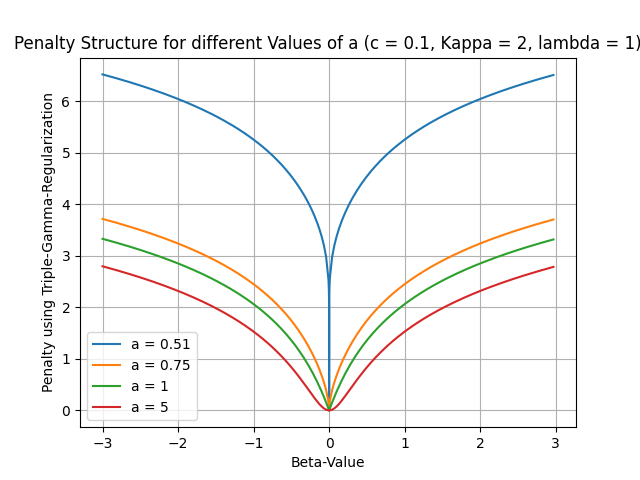
\includegraphics[scale=0.75]{../02_simulation/021_simulation_figures/TGPenalty_ChangeInA.png}
\caption{Triple-Gamma-Penalty using different values of $a^\xi$}
\label{fig:VariationInA}
\end{figure}

Seeing this, it is apparent that a value of $a^\xi$ close but strictly larger that $0.5$ mimics the behaviour of the \textit{Arctan Penalty} by \textcite{WangZhu2016} in small neighbourhoods of $\beta=0$. Similar, large positive values for $a^\xi$ lead to a \textit{Gaussian Penalty} like behaviour in small neighbourhoods of $\beta = 0$ as recently proposed by \textcite{JohnVettamWu2022}.\\
\newpage

\textit{Variations of the Hyperparameter $c^\xi$}\\

In contrast to the hyperparameter $a^\xi$, which mainly affects the behaviour at and around $\beta=0$, changes in $c^\xi$ mainly affect the behaviour in the tails. However, the effect that a change in $c^\xi$ has on the penalty structure can be split up in two rough subsets of $(0,\infty)$. The effect of the first subset of values for $c^\xi$ which are strictly greater than $0$ but less or equal than $0.1$ can be found in figure \ref{fig:ChangeInC_SmallValues} (as already mentioned before, by definition, $c^\xi$ has to be strictly greater than zero: $c^\xi > 0$). Here, it can be seen that as the values for $c^\xi$ become smaller, a shifting effect takes place which generally does not influence the overall structure of the penalty, but increases the amount of penalty which is added to the risk function for $\beta$-values which are different from zero (In a sense, this has a similar effect to changes in $\kappa_B$, which will be explained later). Or, to put it differently, with values of $c^\xi$ closer to zero, the data has be become even more convincing that the value is significantly different from zero.\\


\begin{figure}[!h]
\centering
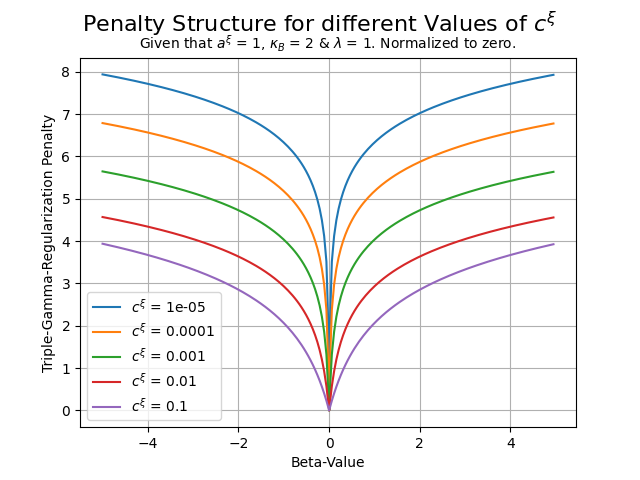
\includegraphics[scale=0.75]{../02_simulation/021_simulation_figures/TGPenalty_ChangeInC_Part2.png}
\caption{Triple-Gamma-Penalty using different values of $c^\xi$ with $0 < c^\xi \leq 0.1$}
\label{fig:ChangeInC_SmallValues}
\end{figure}

However, the more interesting effect that a change in $c^\xi$ has on the penalty structure can be seen for values of $c^\xi$ that are greater than $0.1$. In figure \ref{fig:ChangeInC_LargeValues}, a plot can be found with the Triple-Gamma-Penalty for larger values of $c^\xi$. Again, starting from the baseline with $c^\xi = 0.1$, higher values for this hyper-parameter mainly change the behaviour of the penalty in the tails. A result that has already been shown by \textcite{TGP2020} in Table 1, where multiple different hyper-parameter settings are presented, is that with an increasing value for $c^\xi$ and with $a^\xi = 1$ as well as $\kappa_B = 2$, the Triple-Gamma-Prior converges to a \textit{LASSO} like shrinkage behaviour. A property which carries over to the proposed regularization setting when using the proposed hyper-parameter values, thus showing that the Triple-Gamma-Penalty can be used both as a non-convex penalty as well as a \textit{LASSO} penalty, creating increased flexibility in modelling approaches. 

\begin{figure}[!h]
\centering
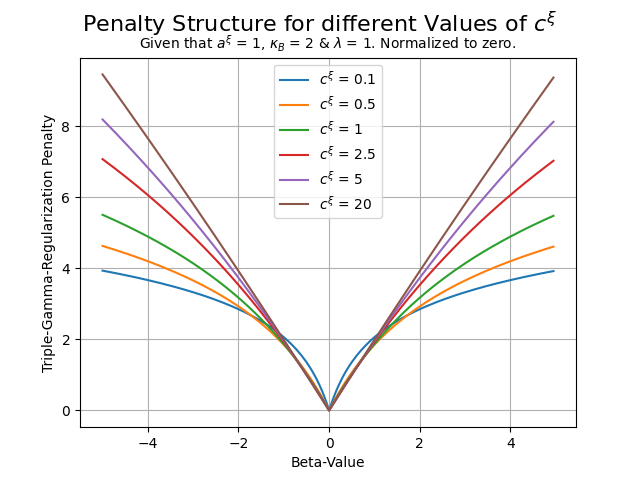
\includegraphics[scale=0.75]{../02_simulation/021_simulation_figures/TGPenalty_ChangeInC_Part1.png}
\caption{Triple-Gamma-Penalty using different values of $c^\xi$ with $c^\xi \geq 0.1$}
\label{fig:ChangeInC_LargeValues}
\end{figure}

\textit{Variations of the Hyperparameter $\kappa_B$}\\

The third and final hyper-parameter $\kappa_B$ enters the Triple-Gamma-Penalty $J_{TG}(\beta)$ as part of $\phi^\xi = \frac{2c^\xi}{\kappa_B^2 a^\xi}$ as can be seen from equation \ref{eq:tgr}. Notably, $\kappa_B$ is squared and thus only the absolute value of $\kappa_B$, $|\kappa_B|$, influences the structure of the penalty. The overall third function value is defined as $\frac{\beta_j^2}{2\phi^\xi}$ and by plugging in $\phi^\xi$ we get $\frac{\beta_j^2\kappa_ B^2a^\xi}{4c^\xi}$, it can be seen that a value of $\kappa_B = 0$ leads to the entire parameter value being zero for all values of $\beta_j$. Hence, a change in $\beta_j$ won't influence the penalty and furthermore won't have an influence on the overall risk minimization problem, the result being that the optimal set of parameters will only depend on the chosen loss function.\\

For all values of $\kappa_B \neq 0$, the value of the hyper-parameter will influence the penalty structure. A plot with several different values for the absolute value of $\kappa_B$ can be found in figure \ref{fig:TGPenalty_ChangeInKappa}. It can be seen that $\kappa_B$ has a scaling effect on the strength of the penalty, thus playing a similar role as the generally multiplicatively added regularization parameter $\lambda$. For small values of $\kappa_B$, the penalty only has a weak singularity in small neighbourhoods around $0$, thus making it more likely for the parameters to be different from zero. As $\kappa_B$ increases, the spike becomes more pronounced and thus increases the added penalty for parameters different from zero. \\

\begin{figure}[h!]
\centering
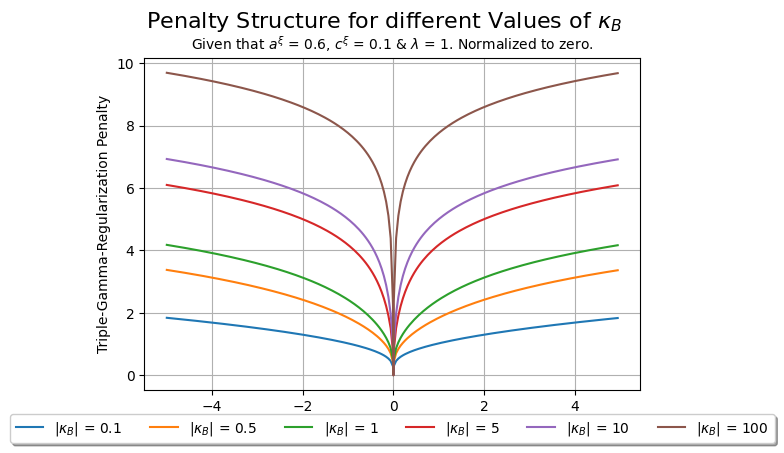
\includegraphics[scale=0.75]{../02_simulation/021_simulation_figures/TGPenalty_ChangeInKappa.png}
\caption{Triple-Gamma-Penalty using different values of $\kappa_B$}
\label{fig:TGPenalty_ChangeInKappa}
\end{figure}

Although it has a scaling effect like $\lambda$, it still has this structural effect as well. Allowing myself to use a Bayesian analogy in this setting, it can be viewed as follows: Increasing $\kappa_B$ corresponds to a way of putting more prior knowledge on zero and thus pulling coefficients stronger towards zero.\\

A summary of all these effects can be found in table \ref{tab:VariationsInHyperparameters} below where the effects of positive and negative changes in the hyperparameters as well as defined ranges for these parameters are defined. 

\newpage
%---- Table Summarizing the Effects of Changes in the Hyperparameters
\begin{landscape}
\hspace{3cm}
\begin{table}[h!]
\centering
\begin{tabular}{lcccccc}\toprule
		& \multicolumn{2}{c}{Change} & \multicolumn{2}{c}{Mathematical Properties}\\
		\cmidrule(r{4pt}){2-3} \cmidrule(l){4-5}
Variable     	& \textbf{Positive} Change  & \textbf{Negative} Change & Defined Range & Misc.\\\midrule
$a^\xi$  	& \makecell{Shifting towards\\ \textit{Gaussian}-like behaviour\\ at $\beta = 0$} & \makecell{Shifting towards singularity\\ at $\beta = 0$; Higher\\ immediate penalty\\ for coefficients\\ $\beta \neq 0$} & $(0.5, \infty)$ & -\\
$c^\xi$ 		& \makecell{Generally, convergence towards \\ convexity and, given certain \\ settings for $a^\xi$ and\\ $\kappa_B$, LASSO. Higher values\\ increase the additional penalty\\ for higher absolute values of $\beta$.} &  \makecell{For values smaller \\ than $0.1$, similar effect\\ to increase in $a^\xi$} & $(0, \infty)$ & - \\
$\kappa_B$ 	& \makecell{The singularity\\ at $\beta=0$ becomes more\\ pronounced, putting more\\ \textit{prior knowledge} on $\beta$\\ being zero.} & \makecell{The reverse effect\\ to the positive effect.} & $(-\infty, \infty)$ & \makecell{When $\kappa_B=0$, the\\ value of $\beta$ doesn't affect\\ the overall penalty anymore,\\ thus reverting the optimization\\ problem back to the\\ non-penalized one.} \\\bottomrule
\end{tabular}
\caption{Summary of the effects of changes in the hyperparameters $a^\xi$, $c^\xi$ and $\kappa_B$ on the penalty structure}
\label{tab:VariationsInHyperparameters}
\end{table}
\end{landscape}

\newpage

\subsection{Comparison to already existing Penalty Terms}\label{subsec:comparepenalties}

As already mentioned in section \ref{sec:litreview}, several other penalty terms have already been widely studied in the literature. Convex penalties like \textit{Ridge} \parencite{HoerlKennard1970a} or non-convex penalties like the \textit{Ar(c)tan} \parencite{WangZhu2016} and \textit{Gaussian} \parencite{JohnVettamWu2022} have managed to establish itself as prominent approaches to regularization. It is now certainly of interest to see how the \textit{Triple-Gamma} penalty compares to the established methods. Seeing that, due to its flexibility, there is not \textit{one} \textit{Triple-Gamma} penalty, three distinct hyper-parameter setting have been chosen to represent the proposed penalty term. 

\begin{table}[h!]
\centering
\begin{tabular}{l|ccc}\toprule
		& \multicolumn{3}{c}{Hyperparameter} \\\cmidrule(r{4pt}){2-4}
     	& $a^\xi$  & $c^\xi$ & $\kappa_B$\\\midrule
Setting 1&	$0.75$	&	$0.1$ &	$2$\\
Setting 2&	$5$  &   $0.01$ & $2$\\
Setting 3&  $0.51$  & $0.001$&$1$\\ \bottomrule
\end{tabular}
\caption{Three Example Settings of the \textit{Triple-Gamma} Penalty}
\label{tab:TGSettings}
\end{table}

A visualisation of these settings can be found in figure \ref{fig:DifferentTGPSettings}. It can be seen that all settings differ heavily in its structure and thus its influence on the optimization problem and in the end the resulting parameters. 

\begin{figure}[H]
\centering
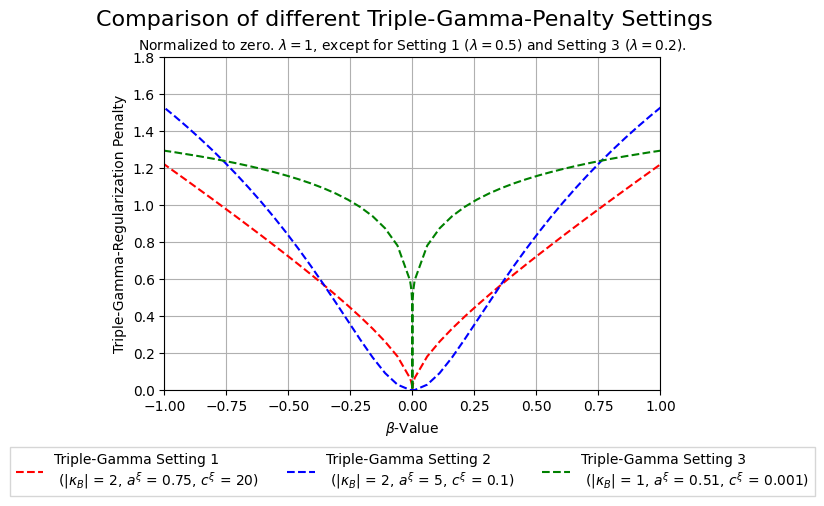
\includegraphics[scale=0.75]{../02_simulation/021_simulation_figures/TGPenalty_DifferentSettings.png}
\caption{Different Settings of the Triple-Gamma-Penalty}
\label{fig:DifferentTGPSettings}
\end{figure}

\textit{Setting 1} is a \textit{LASSO} like regularization penalty, but still keeps the non-convex shape of the Triple-Gamma penalty. \textit{Setting 2} introduces the smooth-at-origin property but keeps a similar shape than \textit{setting 1} in the tails. \textit{Setting 3} has the most distinct structure with a strong singularity at origin but tails which fall of very quickly and thus adds relatively little penalty for parameters that are above $1$ in absolute terms.\\

\begin{figure}[h!]
\centering
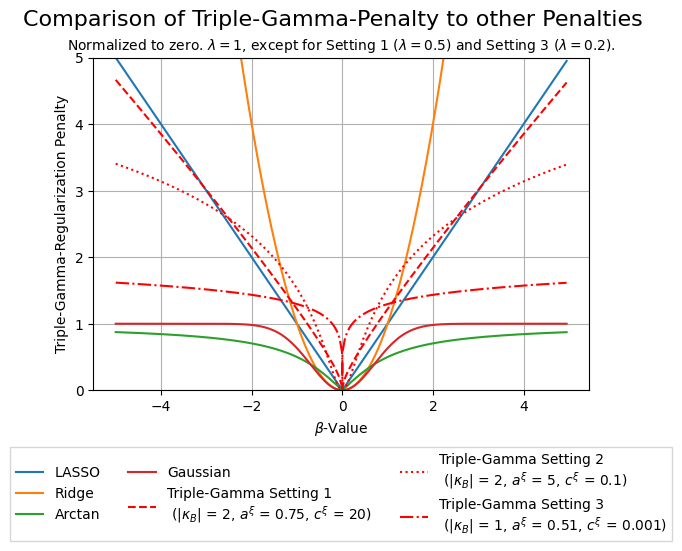
\includegraphics[scale=0.75]{../02_simulation/021_simulation_figures/TGPenalty_Comparison.png}
\caption{Basic Representation of the Triple-Gamma-Penalty using Hyperparameters $c^\xi = 0.1, \kappa_B = 2, a^\xi = 0.75$ compared to \textit{LASSO} and \textit{Ridge} Penalties}
\label{fig:DifferentPenalties}
\end{figure}

Additionally, a comparison of these \textit{Triple-Gamma} settings to a selection of other regularization penalties can be found in figure \ref{fig:DifferentPenalties}. As can be seen here, \textit{setting 1} of the \textit{Triple-Gamma} penalty imitates a \textit{LASSO} penalty with a slightly decreasing additional penalty, resulting in a weakened bias which is common to \textit{LASSO} estimates. \textit{Setting 3} has a similar structure than the non-convex penalties \textit{Gaussian} and \textit{Arctan}, but with a string singularity at zero. Here, it can clearly be seen that the \textit{Triple-Gamma} penalty is not a penalty which converges in the tails, as do \textit{Gaussian} and \textit{Arctan}, but still has a considerably weaker bias as convex methods like \textit{LASSO} and \textit{Ridge}. Overall, figure \ref{fig:DifferentPenalties} showcases the variety of possible penalties that can be implemented using the \textit{Triple-Gamma} penalty. 


%\subsection{Alternative Specification (with +1 to mimic artan)}

%Before moving on to the simulation study in section \ref{sec:simstudy_overall}, this might be the suitable place in this thesis to elaborate on a related concept. As previously mentioned, the \textit{Arctan} penalty developed by \textcite{WangZhu2016} has a similar structure as the \textit{Triple-Gamma-Penalty} in small neighbourhoods near $\beta = 0$ when using specific hyper-parameters (see section \ref{subsec:comparepenalties}). The distinctive structural difference between these two penalties emerge when looking at the limits when  $\underset{\beta \to +/- \infty}{\lim J_{TG}(\beta)}$

%\begin{lightbluebox}
%Propose different concepts?
%\end{lightbluebox}


%----- Simulation Section
\newpage
\section{Simulation Study}\label{sec:simstudy_overall}
To test the proposed method of section \ref{sec:modelderivation} a simulation study will now be conducted whether, and if so, in what scenarios, the \textit{Triple-Gamma} penalty might be valuable addition to the literature. Of course several previously introduced methods have also been tested using simulation studies, but the methodology behind these studies usually varies from paper to paper. However, before moving on to this section of the thesis, the question remains on how to solve the optimization problem in \ref{eq:tgr}. 

\subsection{Approaches to Estimation}
As already mentioned in chapter \ref{sec:litreview}, non-convex penalties like the \textit{Triple-Gamma} penalty are usually harder to solve than convex optimization problems. The reason being that convex functions have a unique global minimum, whereas non-convex functions can have multiple local minima, which are not necessarily a global minimum. \MC In addition, unlike for example \textit{Ridge} regression, the \textit{Triple-Gamma} penalty like many other established penalties in the literature does not have a closed form solution for this optimization problem. Thus, it is necessary to apply an optimization algorithm which solves this problem iteratively. An algorithm which has established itself to solve these kinds of problems is called \textit{Gradient Descent} \parencite[229--248]{GrippoSciandrone2023}. In its essence, the algorithm tries to minimize a loss function by iteratively adjusting the model parameters in the direction that reduces the loss most. It calculates the gradient of the loss function with respect to the model parameters and then updates the parameters by a learning rate. This iterative process can either be repeated until a specified number of iterations is reached or a local (or global) minimum has been found. As already mentioned, this can lead to problems when dealing with non-convex optimization problems as multiple local minima might exist, which do not necessarily need to be global ones. Various approaches to deal with this have been proposed. One method uses random starting points to cover various areas of the optimization space to cover potential multiple local minima. Another method is called \textit{Stochastic Gradient Descent (SGD)} and uses different batches of the dataset to estimate the model parameters \parencite{Amari1993}. The \textit{Gradient Descent} method will be used for the simulation study in the following chapter.\\

For the sake of completeness and as a stepping stone for further research, it is necessary to mention a different approach to solve the optimization problem which is called \textit{Local Linear Approximation (LLA)} algorithm and has been proposed by \textcite{ZouLi2008}. Their resulting \textit{one-step LLA estimates} have several computational advantages and "alleviate the computation burden in the iterative algorithm and overcome the potential local maxima problem in maximizing the nonconcave penalized likelihood" \parencite{ZouLi2008}. Still, to the best of my knowledge, no easily accessible programming packages exist for this algorithm.

\subsection{Scenario Simulation}
Various simulation studies comparing different regularization penalties have been published so far. \textcite{VettamJohn2022} for example have compared \textit{LASSO, Ridge, MCP, SCAD, Laplace} and \textit{Arctan} in the context of the estimation of neural networks. \textcite{WangEtAl2020} have tested a range of penalties in the context of linear models and analysed various the performance of penalties using levels of sparsity, dimensionality and data availability. The authors tested the performance based on three criteria: \textit{prediction}, \textit{variables selection} and \textit{variables ranking}. This simulation study will focus on the the first of these metrics.\\

\textit{Prediction} is usually measured by splitting a simulated dataset into a training dataset and a test dataset. The model is fitted on the training dataset and then tested on the test dataset using a metric like the \textit{mean squared error (MSE)}. \textit{\textit{Variable Selection} is measured in various ways. \textcite{WangEtAl2020} used \textit{true-positive} and \textit{false-positive} rates as their metric of choice. As several of the tested methods in this simulation study do not perform variable selection naturally due to its \textit{smooth-at-origin} property and thus report estimates larger than zero, a different metric will be chosen for this simulation study. To test whether models accurately predict the underlying data generating process and also result in estimates close to its true coefficients, the square of the absolute deviation between the true coefficient and the estimated coefficient of each variable will be computed and summed up. Using this metric, models whose estimates are close the true coefficients will perform than models whose estimates are far off.\\}
\begin{lightbluebox}
Some of the previous paragraph is in italic, because I initially planned on running a second simulation study on this metric as well, but implementation and runtime issues made it difficult. Will probably just mention it. 
\end{lightbluebox}

To evaluate the models in a wide range of contexts, every simulation scenario will vary in terms off three variables: \textit{sample size $N$} (ie $N=100$ meaning that for every run, a total of $100$ observations will be generated), \textit{dimensionality $p$} (ie $p=10$ meaning a total of ten covariates will included in the model) and \textit{sparsity $s$} (ie $s=0.1$ meaning that 10\% of the covariates have a true coefficients different from zero). The set of values chosen for each scenario variable can be found in table \ref{tab:Scenarios}. Using this values, all possible combinations of these variable settings will be formed, resulting in a total of $36$ possible scenarios. 

\begin{table}[h!]
\begin{center}
\begin{tabular}{lc}\toprule
Variable & Values\\\midrule
Sample Size $N$ & $10, 100, 250$\\
Dimensionality $p$ & $10, 50, 200$\\
Sparsity $s$ & $0.1, 0.5, 0.9$\\\bottomrule
\end{tabular}
\caption{Scenarios Values}
\label{tab:Scenarios}
\end{center}
\end{table}

The remaining issue to cover deals with the weighting/regularization parameter $\lambda$ (see section \ref{sec:theorysuper}) and how it is set. This key parameter controlling the strength of the influence of the penalty on the overall optimization result is usually set by the user, however another \textit{hands-off} method is cross-validation, which will be used for this simulation \parencite[250--251]{ESL2009}. A grid of possible values for $\lambda$ is chosen, the model is being estimated for every possible value, and the best model will be chosen based on the chosen cross-validation metric. For this simulation study, all values between $0$ and $1$ based on $0.01$ steps will be tested on the first generated dataset. To save time when it comes to computation, the search will be stopped if the chosen metric hasn't improved for more than 10 new values for $\lambda$. After his run, these optimal values will be used in the overall simulation. \textbf{For the application of the gradient descent algorithm a maximum number of 750 epochs has been set.} The simulations have been run with Python (Version 3.11.4) along with scikit-learn (Version 1.4.1.post1) and PyTorch (Version 2.2.2).\footnote{More information on the packages used and its installed version can be found in the accompanying GitHub repository.}

\subsection{Simulation Study} 

For the simulation study testing the models prediction accuracy the key metric to test performance will be the \textit{mean-squared-error (MSE)}. The data is being generated the following way: Given a set of scenario parameters $N_i$, $p_i$ and $sd_i$, the first $s_i*p_i$ coefficients, rounded to the next larger integer, will be set to $3$ and the remaining will be set to $0$. Then, $N_i$ draws will be generated from a normal distribution with mean $0$ and variance $1$ for each of the $p_i$ features. Using these coefficients and the data from the features a response variable $y$ will be computed and noise generated from a normal distribution with mean $0$ and variance $\sigma_i$. According to \textcite{WangEtAl2020}, the respective $\sigma_i$ will be computed based on the \textit{Signal-To-Noise Ration (SNR)}. The \textit{SNR} is given by $SNR = \sqrt{\beta^TX^TX\beta/(N_i\sigma_i^2)}$ and by setting the \textit{SNR} to a specific value, one can adjust how string the noise in the data is relative to the sound of the actual data generating process. For the purpose of this study, and similar to \textcite{WangEtAl2020}, a \textit{SNR} equal to one will be used. In terms of the regularization parameter $\lambda$, the search for the optimal $\lambda$ will be performed by using five-fold-cross-validation on the a set of possible $\lambda$ values. For every method and every run in every scenario separately, the optimal $\lambda^*_i$ will be chosen which generates the lowest validation loss on the testset. This grid-serach procedure will be performed for every $\lambda_i \in \{0.001, 0.01, 0.1, 0.25, 0.4, 0.5, 0.6, 0.75, 0.9, 0.95\}$.\\

Using the set of scenario variables mentioned in table \ref{tab:Scenarios}, all possible combinations will be formed resulting in the overall $27$ scenarios. The code iterates through the list of scenarios, generates 15 datasets based on these scenarios variables and all tested methods will be estimated on every one the test part of these datasets. Afterwards, the validation loss will be computed for each method and stored. This procedure results in tables \ref{tab:PredSim}, which shows the mean and standard deviation of the distribution of the validation loss for every scenario and every method. The values colored in \textcolor{red}{red} indicate the smallest means for every scenario. Before advancing to the overall results of this simulation study, it might be useful to have a look at a specific scenario to better understand the results in table \ref{tab:PredSim}, which will be the scenario with $N=100, p=200, s=0.1$.\\

In this scenario, we are dealing with a dataset of $100$ observations, $200$ features and $20$ non-zero coefficients.\footnote{$200 \times 0.1 = 20$.} A figure with boxplots showcasing the distributions of the Mean-Squared-Error rates on the validation set for all methods can be found in figure \ref{fig:SpecificScenario}.

\begin{figure}[h!]
\centering
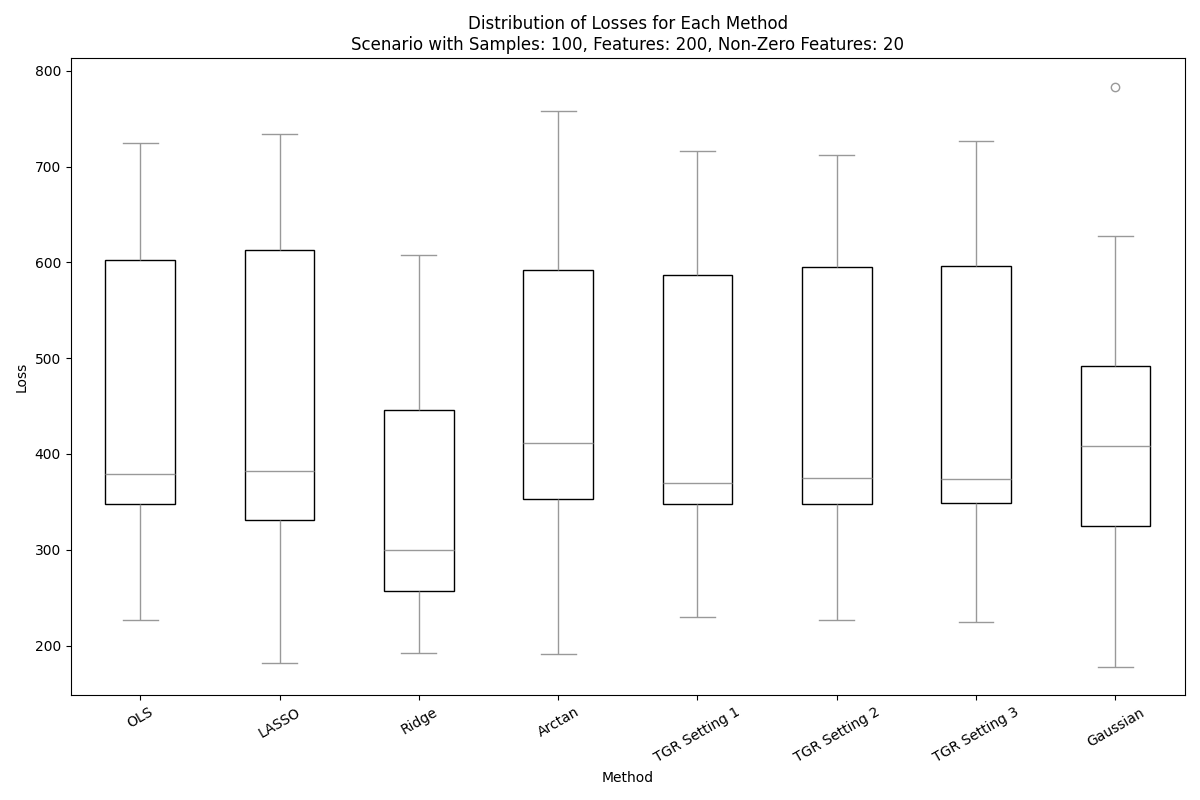
\includegraphics[scale=0.5]{../02_simulation/021_simulation_figures/Scenarion_100_200_20.png}
\caption{Distribution of MSE on Validation Set in the Scenario with $100$ Observations, $25$ Features and $3$ non-zero Coefficients}
\label{fig:SpecificScenario}
\end{figure} 	

This scenario, which is a good exmaple for a sparse scenario, where a lot of features are in the dataset but only a small part of it is different from zero, i.e. has an effect on the outcome. Here, \textit{Ridge} performs best by far in manages to produce the smallest mean in loss with about $300$. Except for \textit{Gaussian}, every method produces a right-skewed distribution indicating that most methods produce average losses of around $400$ most of the time with common outliers up to $750$.  

An overview of the results for each of the $27$ scenarios can be found in table \ref{tab:bestmethod}. In the left half of the table the scenario parameters are presented and in the right half the best method based on the method having the lowest mean as well as median validation loss. In general, the results confirm the results from \textcite{WangEtAl2020} that no go-to method in regularization have been found. In terms of the mean loss, \textit{LASSO}, \textit{Ridge}, \textit{Gaussian} and \textit{Arctan} have managed to perform best in one or more scenarios. When it comes to the median, \textit{LASSO}, \textit{Setting 1 and 2 of the TGR}, \textit{Ridge}, \textit{Arctan} and \textit{Gaussian} have managed to perform best in one or more scenarios. Clearly, no one single method stands out as an overall winner in this simulation. However, these results have to be taken with care as will be discussed in section \ref{sec:crit} later on. 

\begin{lightbluebox}
I will extend my discussion on the results and go a bit more into detail. But the general idea of the results should be there.
\end{lightbluebox}

\begin{table}[h!]
\begin{center}
\begin{tabular}{ccc|l|l}
\toprule
\multicolumn{3}{c}{Scenario Parameters} & \multicolumn{2}{c}{Moment}\\
\midrule
Samples & Features & Non-Zero Features & Best Method (Mean) & Best Method (Median) \\
\midrule
10 & 10 & 1 & LASSO & LASSO \\
10 & 10 & 5 & Ridge & TGR Setting 1 \\
10 & 10 & 9 & Ridge & Ridge \\
10 & 50 & 5 & Ridge & Ridge \\
10 & 50 & 25 & Gaussian & Gaussian \\
10 & 50 & 45 & Ridge & Ridge \\
10 & 200 & 20 & Gaussian & Arctan \\
10 & 200 & 100 & Arctan & LASSO \\
10 & 200 & 180 & Gaussian & Gaussian \\
100 & 10 & 1 & Arctan & Arctan \\
100 & 10 & 5 & Gaussian & Gaussian \\
100 & 10 & 9 & Gaussian & Ridge \\
100 & 50 & 5 & Gaussian & Gaussian \\
100 & 50 & 25 & Ridge & Ridge \\
100 & 50 & 45 & Ridge & Ridge \\
100 & 200 & 20 & Ridge & Ridge \\
100 & 200 & 100 & Gaussian & Ridge \\
100 & 200 & 180 & Ridge & Ridge \\
250 & 10 & 1 & Gaussian & Gaussian \\
250 & 10 & 5 & Gaussian & Gaussian \\
250 & 10 & 9 & Gaussian & TGR Setting 2 \\
250 & 50 & 5 & Gaussian & Gaussian \\
250 & 50 & 25 & Ridge & Ridge \\
250 & 50 & 45 & Ridge & Ridge \\
250 & 200 & 20 & Ridge & Ridge \\
250 & 200 & 100 & Ridge & Ridge \\
250 & 200 & 180 & Ridge & Ridge \\
\bottomrule
\end{tabular}
\caption{Table showing the best performing methods according to smallest Mean and Median Loss accordingly}
\end{center}
\label{tab:bestmethod}
\end{table}


\newpage
\subsection{Computational Efficiency}
At this point of the thesis it is necessary to quickly cover the topic of computational efficiency. As mentioned earlier, this simulation study has been implemented using Python along with PyTorch. As the \textit{Triple-Gamma} penalty is not a simple algebraic computation, as for example computing the absolute value of a real number in the case of \textit{LASSO} or computing the arcus tangens in the case of the \textit{Arctan} penalty, it is apparent that the computation of the loss function given a set of parameters is not very straight-forward and computationally expensive. In its current implementation, the Python function computing the \textit{Triple-Gamma-Loss} has to access a second function which approximates the logarithm of the confluent hyper-geometric  function of the second kind. More importantly, it does so for every parameter in the model. This is, to no surprise, very inefficient and makes computations in high dimensions unnecessarily complicated. In figure \ref{fig:ComputationTime} a plot can be found which shows the time to estimate all three settings of the \textit{Triple-Gamma-Regularization} on a dataset generated with parameters $N=100$ and $s=0.1$ with an increasing number of features $p$.\\

It is also worth noting that the compuational efficiency of the \textit{Triple-Gamma-Penalty} still relies on the specification of the penalty. \textit{Setting 2} for example with its very \textit{smooth-at-origin} behaviour takes significantly longer to compute compared to its \textit{singular-at-origin} specifications in \textit{setting 1} and \textit{setting 3}.


\begin{figure}[h!]
\centering
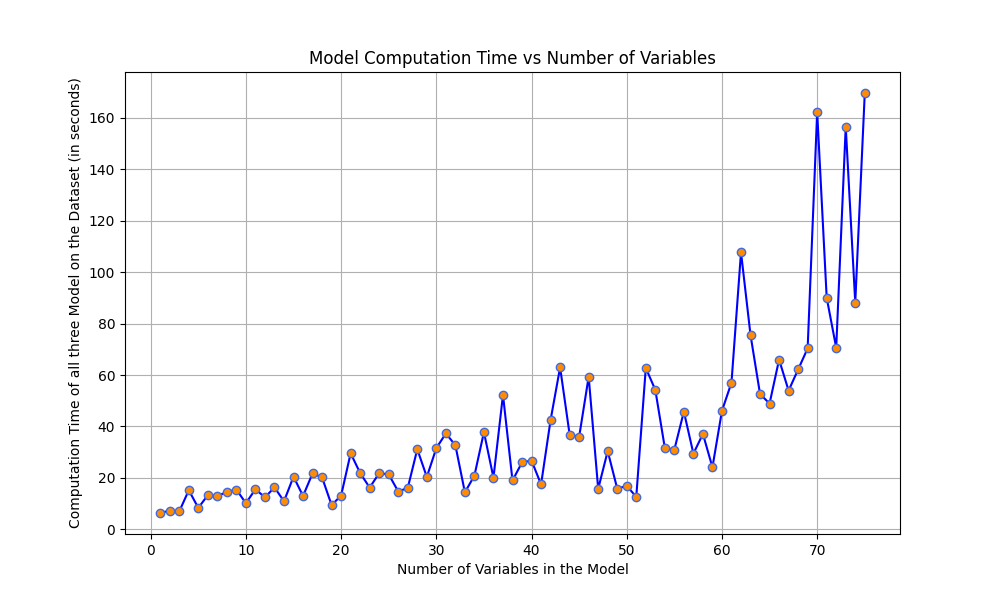
\includegraphics[scale=0.55]{../02_simulation/021_simulation_figures/ComputationTime_Example.png}
\caption{Time necessary to compute all three scenarios of the Triple-Gamma-Regularization with $N=100$ and $s=0.1$ dependent on the number of Features $p$}
\label{fig:ComputationTime}
\end{figure} 	

As can be seen from figure \ref{fig:ComputationTime} above, the time to estimates these models increases drastically with an increased number of variables. Setting aside that it might even grow exponentially, it can be seen that the computation time also increasingly becomes more unstable. Several approaches might help in resolving these issues, like optimizing the underlying approximation of the confluent hypergeometric funciton or choosing a different estimation algorithm altogether (see section 6.1). Another approach could be to implement the underlying estimation in a more efficient programming language when it comes to runtime like C++. All in all, this definitely opens up a field for further research to make the overall method more suitable for application. 

\begin{landscape}
\begin{longtable}{lllllllllllrrrrrrrr}
\toprule
\caption{Mean and Standard Deviations of MSE on the Validation Set for different Scenarios (15 runs per scenario)} \\
\toprule
\makecell{\textbf{Sample} \\ \textbf{Size}} & \makecell{\textbf{Features}} & \makecell{\textbf{Non-zero} \\ \textbf{Features}} & \makecell{\textbf{OLS}} & \makecell{\textbf{LASSO}} & \makecell{\textbf{Ridge}} & \makecell{\textbf{TGR} \\ \textbf{Setting 1}} & \makecell{\textbf{TGR} \\ \textbf{Setting 2}} & \makecell{\textbf{TGR} \\ \textbf{Setting 3}} & \makecell{\textbf{Arctan}} & \makecell{\textbf{Gaussian}} \\
\midrule
\endhead
\midrule \multicolumn{11}{r}{{Continued on next page}} \\
\endfoot

\bottomrule
\endlastfoot

\multicolumn{11}{c}{{\tablename\ \thetable{} -- continued from previous page}} \\
\toprule
\makecell{\textbf{Sample} \\ \textbf{Size}} & \makecell{\textbf{Features}} & \makecell{\textbf{Non-zero} \\ \textbf{Features}} & \makecell{\textbf{OLS}} & \makecell{\textbf{LASSO}} & \makecell{\textbf{Ridge}} & \makecell{\textbf{TGR} \\ \textbf{Setting 1}} & \makecell{\textbf{TGR} \\ \textbf{Setting 2}} & \makecell{\textbf{TGR} \\ \textbf{Setting 3}} & \makecell{\textbf{Arctan}} & \makecell{\textbf{Gaussian}} \\
\midrule
\endfirsthead

% &  &  &  Arctan &  Gaussian &  LASSO &  OLS &  Ridge &  TGR Setting 1 &  TGR Setting 2 &  TGR Setting 3 & median Arctan & median Gaussian & median LASSO & median OLS & median Ridge & median TGR Setting 1 & median TGR Setting 2 & median TGR Setting 3 \\
%Samples & Features & Non-Zero Features &  &  &  &  &  &  &  &  &  &  &  &  %&  &  &  &  \\
\midrule
\multirow[t]{9}{*}{100} & \multirow[t]{3}{*}{10} & 1 & \makecell{8.143 \\ (2.511)} & \makecell{10.027 \\ (3.428)} & \makecell{8.516 \\ (2.645)} & \makecell{8.761 \\ (2.474)} & \makecell{9.398 \\ (2.78)} & \makecell{8.76 \\ (2.475)} & \makecell{8.76 \\ (2.474)} & \makecell{8.762 \\ (2.475)} \\
 &  & 5 & \makecell{55.223 \\ (20.503)} & \makecell{50.321 \\ (17.244)} & \makecell{55.148 \\ (19.635)} & \makecell{55.609 \\ (20.961)} & \makecell{56.055 \\ (19.489)} & \makecell{55.609 \\ (20.964)} & \makecell{55.61 \\ (20.962)} & \makecell{55.609 \\ (20.965)}  \\
 &  & 9 & \makecell{94.411 \\ (20.534)} & \makecell{91.228 \\ (33.291)} & \makecell{94.499 \\ (21.804)} & \makecell{94.328 \\ (20.518)} & \makecell{91.867 \\ (22.567)} & \makecell{94.327 \\ (20.518)} & \makecell{94.323 \\ (20.517)} & \makecell{94.331 \\ (20.516)} \\
\cline{2-19}
 & \multirow[t]{3}{*}{200} & 100 & \makecell{2226.539 \\ (739.514)} & \makecell{1827.873 \\ (444.322)} & \makecell{2208.412 \\ (787.768)} & \makecell{2216.253 \\ (723.275)} & \makecell{1830.305 \\ (737.83)} & \makecell{2216.27 \\ (728.55)} & \makecell{2212.339 \\ (723.82)} & \makecell{2219.283 \\ (725.999)}  \\
 &  & 180 & \makecell{3646.99 \\ (772.852)} & \makecell{3715.863 \\ (938.21)} & \makecell{3636.415 \\ (839.114)} & \makecell{3599.837 \\ (815.794)} & \makecell{2946.407 \\ (597.781)} & \makecell{3606.205 \\ (814.385)} & \makecell{3601.481 \\ (818.954)} & \makecell{3597.845 \\ (812.657)}  \\
 &  & 20 & \makecell{445.823 \\ (159.82)} & \makecell{416.379 \\ (171.003)} & \makecell{431.558 \\ (169.15)} & \makecell{442.394 \\ (155.412)} & \makecell{348.24 \\ (139.308)} & \makecell{438.987 \\ (151.256)} & \makecell{440.075 \\ (151.842)} & \makecell{441.839 \\ (153.669)}  \\
\cline{2-19}
 & \multirow[t]{3}{*}{50} & 25 & \makecell{432.699 \\ (197.61)} & \makecell{481.517 \\ (180.227)} & \makecell{368.908 \\ (162.292)} & \makecell{443.575 \\ (194.823)} & \makecell{339.177 \\ (125.94)} & \makecell{444.025 \\ (194.793)} & \makecell{443.355 \\ (194.348)} & \makecell{443.488 \\ (194.801)} \\
 &  & 45 & \makecell{836.618 \\ (324.041)} & \makecell{814.207 \\ (342.009)} & \makecell{721.727 \\ (251.258)} & \makecell{846.918 \\ (337.334)} & \makecell{614.541 \\ (170.535)} & \makecell{846.84 \\ (337.454)} & \makecell{846.12 \\ (337.28)} & \makecell{846.476 \\ (336.935)}  \\
 &  & 5 & \makecell{93.694 \\ (47.708)} & \makecell{67.294 \\ (34.223)} & \makecell{71.908 \\ (25.233)} & \makecell{121.977 \\ (59.6)} & \makecell{79.943 \\ (23.445)} & \makecell{121.636 \\ (59.986)} & \makecell{121.991 \\ (59.878)} & \makecell{121.864 \\ (60.022)} \\
\cline{1-19} \cline{2-19}
\multirow[t]{9}{*}{10} & \multirow[t]{3}{*}{10} & 1 & \makecell{11.91 \\ (17.701)} & \makecell{28.907 \\ (43.717)} & \makecell{8.635 \\ (10.314)} & \makecell{15.504 \\ (18.187)} & \makecell{9.851 \\ (10.121)} & \makecell{16.438 \\ (16.91)} & \makecell{16.028 \\ (17.231)} & \makecell{16.369 \\ (17.874)}\\
 &  & 5 & \makecell{143.56 \\ (167.634)} & \makecell{177.867 \\ (209.043)} & \makecell{94.755 \\ (76.06)} & \makecell{141.116 \\ (171.209)} & \makecell{75.967 \\ (54.791)} & \makecell{138.544 \\ (160.823)} & \makecell{140.159 \\ (163.716)} & \makecell{138.335 \\ (165.406)} \\
 &  & 9 & \makecell{262.25 \\ (426.742)} & \makecell{201.942 \\ (170.517)} & \makecell{226.472 \\ (407.698)} & \makecell{267.779 \\ (417.718)} & \makecell{200.697 \\ (357.116)} & \makecell{264.61 \\ (412.264)} & \makecell{266.555 \\ (410.478)} & \makecell{267.376 \\ (415.85)} \\
\cline{2-19}
 & \multirow[t]{3}{*}{200} & 100 & \makecell{1808.579 \\ (2076.395)} & \makecell{2980.261 \\ (2754.132)} & \makecell{1808.738 \\ (2060.886)} & \makecell{1838.216 \\ (2040.237)} & \makecell{1834.696 \\ (2044.349)} & \makecell{1835.863 \\ (2057.228)} & \makecell{1834.512 \\ (2033.185)} & \makecell{1837.199 \\ (2046.792)} \\
 &  & 180 & \makecell{4330.096 \\ (4779.502)} & \makecell{2342.614 \\ (2243.02)} & \makecell{4156.453 \\ (4253.531)} & \makecell{4340.759 \\ (4767.094)} & \makecell{4325.067 \\ (4751.866)} & \makecell{4356.129 \\ (4776.532)} & \makecell{4355.088 \\ (4763.186)} & \makecell{4365.29 \\ (4769.61)} \\
 &  & 20 & \makecell{593.649 \\ (857.827)} & \makecell{244.895 \\ (281.378)} & \makecell{590.32 \\ (849.003)} & \makecell{599.976 \\ (833.877)} & \makecell{597.436 \\ (838.781)} & \makecell{590.162 \\ (821.858)} & \makecell{600.672 \\ (838.178)} & \makecell{594.873 \\ (848.782)} \\
\cline{2-19}
 & \multirow[t]{3}{*}{50} & 25 & \makecell{388.054 \\ (321.434)} & \makecell{324.916 \\ (308.065)} & \makecell{364.883 \\ (312.231)} & \makecell{360.303 \\ (306.296)} & \makecell{354.606 \\ (301.023)} & \makecell{362.582 \\ (309.18)} & \makecell{360.177 \\ (305.899)} & \makecell{359.78 \\ (306.077)} \\
 &  & 45 & \makecell{895.964 \\ (794.069)} & \makecell{993.069 \\ (979.897)} & \makecell{898.587 \\ (810.784)} & \makecell{898.939 \\ (794.377)} & \makecell{885.455 \\ (745.737)} & \makecell{908.628 \\ (782.478)} & \makecell{906.609 \\ (780.218)} & \makecell{908.734 \\ (788.112)} \\
 &  & 5 & \makecell{77.59 \\ (72.053)} & \makecell{120.175 \\ (149.159)} & \makecell{74.652 \\ (76.395)} & \makecell{72.223 \\ (70.693)} & \makecell{72.033 \\ (72.748)} & \makecell{74.309 \\ (72.165)} & \makecell{75.892 \\ (73.834)} & \makecell{74.12 \\ (70.883)} \\
\cline{1-19} \cline{2-19}
\multirow[t]{9}{*}{250} & \multirow[t]{3}{*}{10} & 1 & \makecell{9.285 \\ (2.219)} & \makecell{8.203 \\ (1.954)} & \makecell{9.376 \\ (2.179)} & \makecell{9.701 \\ (2.323)} & \makecell{9.704 \\ (2.302)} & \makecell{9.701 \\ (2.323)} & \makecell{9.701 \\ (2.323)} & \makecell{9.701 \\ (2.323)} \\
 &  & 5 & \makecell{50.568 \\ (8.659)} & \makecell{44.651 \\ (7.361)} & \makecell{50.586 \\ (9.112)} & \makecell{51.251 \\ (8.933)} & \makecell{51.128 \\ (9.263)} & \makecell{51.251 \\ (8.933)} & \makecell{51.251 \\ (8.933)} & \makecell{51.251 \\ (8.933)} \\
 &  & 9 & \makecell{92.956 \\ (26.567)} & \makecell{87.92 \\ (20.76)} & \makecell{92.847 \\ (26.272)} & \makecell{92.857 \\ (26.528)} & \makecell{93.317 \\ (25.737)} & \makecell{92.857 \\ (26.528)} & \makecell{92.856 \\ (26.529)} & \makecell{92.857 \\ (26.529)} \\
\cline{2-19}
 & \multirow[t]{3}{*}{200} & 100 & \makecell{2191.822 \\ (464.342)} & \makecell{2207.572 \\ (460.284)} & \makecell{1783.244 \\ (466.102)} & \makecell{2256.102 \\ (467.37)} & \makecell{1397.03 \\ (284.985)} & \makecell{2255.161 \\ (465.895)} & \makecell{2256.095 \\ (466.639)} & \makecell{2256.174 \\ (465.94)} \\
 &  & 180 & \makecell{4037.567 \\ (847.844)} & \makecell{4017.374 \\ (704.43)} & \makecell{3477.884 \\ (714.527)} & \makecell{4083.589 \\ (859.518)} & \makecell{2554.422 \\ (614.084)} & \makecell{4081.027 \\ (859.12)} & \makecell{4082.227 \\ (861.805)} & \makecell{4080.481 \\ (860.907)} \\
 &  & 20 & \makecell{374.787 \\ (102.866)} & \makecell{292.05 \\ (66.283)} & \makecell{282.808 \\ (73.489)} & \makecell{479.24 \\ (121.248)} & \makecell{281.375 \\ (56.671)} & \makecell{479.953 \\ (121.219)} & \makecell{479.651 \\ (120.956)} & \makecell{479.596 \\ (121.574)} & \\
\cline{2-19}
 & \multirow[t]{3}{*}{50} & 25 & \makecell{303.069 \\ (66.83)} & \makecell{304.353 \\ (83.207)} & \makecell{296.789 \\ (68.898)} & \makecell{303.902 \\ (61.62)} & \makecell{289.719 \\ (63.05)} & \makecell{303.919 \\ (61.637)} & \makecell{303.9 \\ (61.61)} & \makecell{303.923 \\ (61.631)} \\
 &  & 45 & \makecell{538.998 \\ (127.705)} & \makecell{565.719 \\ (125.848)} & \makecell{532.489 \\ (129.833)} & \makecell{534.825 \\ (125.456)} & \makecell{502.432 \\ (130.652)} & \makecell{534.794 \\ (125.417)} & \makecell{534.832 \\ (125.462)} & \makecell{534.779 \\ (125.407)}  \\
 &  & 5 & \makecell{55.19 \\ (12.429)} & \makecell{43.153 \\ (10.311)} & \makecell{53.335 \\ (12.516)} & \makecell{66.509 \\ (10.663)} & \makecell{63.255 \\ (13.669)} & \makecell{66.512 \\ (10.667)} & \makecell{66.512 \\ (10.664)} & \makecell{66.516 \\ (10.66)} \\
\cline{1-19} \cline{2-19}
\bottomrule
\end{longtable}
\label{tab:PredSim}
\end{landscape}

%\subsection{Simulation Study for Variable Selection}

%As described in the introductory part of this section, the variable selection part of the simulation study will explore how accurately specific models can estimate the underlying data generating process without worrying about predictive power on a test dataset. Thus, no validation set will be used to measure performance, but rather the deviation of the estimated coefficients to the true data generating coefficients. To showcase this overall procedure, the scenario 

\subsection{Implementation as Python Package}
As mentioned before, this simulation study has been run using Python (Version 3.11.4) along with scikit-learn (Version 1.4.1.post1) and PyTorch (Version 2.2.2). The accompanying code, a list of packages used and its version and other material can be found on \href{https://github.com/therealLucasPaul/MScThesis_Econ}{GitHub}. The script \textit{tgr.py} can be used as a script to apply \textit{Triple-Gamma-Regularization} on a dataset of choice. To make its application easier, the following subsections provides important information on how to use it.

\subsubsection*{General Functions}

\begin{longtable}{|p{4cm}|p{9cm}|}
\hline
\textbf{Function Name} & \textbf{Description} \\
\hline
\endfirsthead

\hline
\textbf{Function Name} & \textbf{Description} \\
\hline
\endhead

\hline
\endfoot

\hline
\endlastfoot

\makecell{\texttt{TripleGamma-}\\\texttt{Regularization}} & Here a class is defining a simple neural network. It uses the \texttt{nn.Module} and initializes a linear model with 10 input features and 1 output feature without an intercept. \\
\hline
	\texttt{TripleGammaReg\_Loss} & This function computes the loss for the Triple Gamma Regularization. It takes the predicted values (\texttt{Y\_HAT}), the true values (\texttt{Y}), the coefficients of the model (\texttt{coefficients}), the regularization parameter (\texttt{lamda}), and the regularization parameters \texttt{a}, \texttt{c} and \texttt{kappa} as input. The loss is computed according to the theoretical formulation by using the script \texttt{log\_hyperu.py}, which approximates the log of the confluent hyper-geometric function of the second kind. \\
\hline
\texttt{TripleGammaModel} & This function trains the \textit{Triple-Gamma} Regularization model. It takes the feature matrix (\texttt{X}), the target values (\texttt{y}), the regularization parameter (\texttt{penalty}), regularization hyper-parameters \texttt{a}, \texttt{c}, \texttt{kappa}, the number of epochs (\texttt{num\_epochs}), and the learning rate (\texttt{lr}) as input. It initializes the \texttt{PyTorch} model and optimizer, uses Gradient Descent to train the model for the specified number of epochs, and returns the trained model, a list of model coefficients for each epoch, and a list of loss values for each epoch.\\
\hline
\end{longtable}

\subsubsection*{Dependencies}
To successfully run the script, the following dependencies are required:
\begin{itemize}
    \item \texttt{torch}: PyTorch library including sub modules \texttt{torch.nn} and \texttt{torch.optim} for building and training neural networks with at least version 2.2.2
    \item \texttt{log\_hyperu as hyperu}: The custom module for computing the logarithm of the hypergeometric function, which can be found on GitHub.
\end{itemize}

\subsubsection*{Data Types of Inputs and Outputs of the Functions}
\begin{itemize}
  	\item \texttt{TripleGammaModel}
    \begin{itemize}
        \item \textbf{Input:} \texttt{X} (Tensor), \texttt{y} (Tensor), \texttt{penalty} (float), \texttt{a} (float), \texttt{c} (float), \texttt{kappa} (float), \texttt{num\_epochs} (int, default=1000), \texttt{lr} (float, default=0.01)
        \item \textbf{Output:} \texttt{model} (Initialization of the class TripleGammaRegularization), \texttt{coef\_list} (list of Tensors), \texttt{loss\_list} (list of Tensors)
    \end{itemize}
\end{itemize}

\section{Possible Extensions and Criticism}\label{sec:crit}

\begin{lightbluebox}
I will write the last two paragraphs as soon as the rest of the thesis is 100\% air tight to avoid having to rewrite the conclusions multiple times. It should take long though.
\end{lightbluebox}
\section{Conclusion}
\begin{lightbluebox}
ENDE
\end{lightbluebox}
\newpage
\section{List of Figures}
\listoffigures

\newpage
\section{List of Tables}
\listoftables

\newpage
\section{References}

\pagenumbering{roman}
\setcounter{page}{\thesavepage}
\pagestyle{plain}
\addcontentsline{toc}{section}{References}
%\bibliographystyle{apalike}
%\bibliography{ref.bib}
\printbibliography[]
\clearpage
\end{document}
